%
%  thesis.tex  2014-08-08  Mark Senn
%
%  This is the root file for a simple example thesis.
%  This example can also be used to prepare a dissertation.
%
%  To make a final copy of your thesis put a '%'
%  in front of the \includeonly command and run:
%    latex thesis
%    latex thesis
%    latex thesis
%    bibtex thesis
%    latex thesis
%    latex thesis
%
%  References cited below:
%
%    TM1996 is short for Thesis Manual 1996.
%    ``A Manual for the Preparation of Graduate Theses'',
%    The Graduate School, Purdue University, 1996.
%
%    TM2006 is short for Thesis Manual 2006.
%    ``A Manual for the Preparation of Graduate Theses'',
%    seventh revised edition, The Graduate School, Purdue University, 2006.
%    http://www.purdue.edu/GradSchool/documents/thesis/graduate-thesis-manual.pdf
%
%  Search for "CHANGE" below and change things as necessary.
%  I recommend putting "%%" before any existing lines that
%  need to be changed and adding your new line(s) immediately
%  below the existing lines.
%

% See
%     http://www.ecn.purdue.edu/~mark/puthesis/#Options
% for documentclass options.
% CHANGE NEXT LINE?
\documentclass[cs,dissertation]{puthesis}

% Define "align" environment used in demo-mathematics.tex.
% CHANGE NEXT LINE?
\usepackage{amsmath}

% Define "multicols" environment environment used in demo-multicols.tex.
% CHANGE NEXT LINE?
\usepackage{multicol}

% Define "subfigure" environment used in "demo-figure.tex".
% CHANGE NEXT LINE?
\usepackage{subfigure}

% Added by KC
\usepackage{hyperref}
\usepackage{xspace}
\usepackage{amssymb}
\usepackage{tikz}
\usepackage{stackrel}
\usepackage{fontenc}
\usepackage{times}
\usepackage{textcomp}
\usepackage{wrapfig}
\newcommand{\ftextrecipe}{{\fontfamily{tmr}\selectfont \textrecipe}}


% Title of thesis (used on cover and in abstract).
% The title shown must be the full, official title of the thesis.
% Superscripts and subscripts are not permitted in the title.
% Reference: TM2006, page 26.
% Use \title{Put Title Here} for a one-line title.
% Use \\ to separate lines in multi-line titles.
% Put % at the end of the last line of a title
% to avoid getting an extra space in the abstract.
% There are two forms of title: one line or more than one line.
% There are examples of both below.
% Only use one \title.
% CHANGE NEXT FIVE LINES.
\title{Functional Programming Abstractions for Weakly Consistent Systems}
% First author name with first name first is used for cover.
% Second author name with last name first is used for abstract.
% Your full name as it appears in the University records appears
% on the cover.
% Reference: TM2006 pages 26, 29.
% There are two forms of author, with and without initials.
% There are examples of both below.
% Only use one \author line.
% CHANGE NEXT TWO LINES.
\author{Sivaramakrishnan Krishnamoorthy Chandrasekaran}{Krishnamoorthy Chandrasekaran, Sivaramakrishnan}

% First is long title of degree (used on cover).
% Second is abbreviation for degree (used in abstract).
% Third is the month the degree was (will be) awarded (used on cover
% and in abstract).
% Last is the year the degree was (wlll be) awarded (used on cover
% and in abstract).
% The degree title for all doctoral candidates is ``Doctor of Philosophy''.
% The precise degree names for master's candidates appear in the list of
% ``Degrees Offered'' in the Graduate School bulletin.
% The date is the month and year that the degree is actually awarded.
% (If you have registered for ``degree only'', revise the thesis title
% page to reflect the new date on which the degree is to be awarded.)
% Reference: TM2006 pages 26--27, 30.
% CHANGE NEXT LINE?
\pudegree{Doctor of Philosophy}{PhD}{Dec}{2014}

% Major professor (used in abstract).
% Use, for example:
%     \majorprof{Sarah Smith}
%     \majorprof{Amy A. Jones}
%     \majorprofs{Sarah Smith and Amy A. Jones}
%     \majorprofs{Sarah Smith, Amy A. Jones, and Lisa B. C. Brown}
% depending on the number of major professors you have.
% CHANGE NEXT LINE.
\majorprof{Suresh Jagannathan}

% Campus (used only on cover)
% Use one of the following:
%     Fort Wayne
%     Hammond
%     Indianapolis
%     West Lafayette
%     Westville
% Reference: TM2006 page 27.
% CHANGE NEXT LINE?
\campus{West Lafayette}


%
% My command definitions not specific to my thesis.
%

% CHANGE NEXT LINE?
%
%  mydefs.tex  2007-03-19  Mark Senn  http://www.ecn.purdue.edu/~mark
%
%  Command definitions that can be used in all documents that have
%      %
%  mydefs.tex  2007-03-19  Mark Senn  http://www.ecn.purdue.edu/~mark
%
%  Command definitions that can be used in all documents that have
%      %
%  mydefs.tex  2007-03-19  Mark Senn  http://www.ecn.purdue.edu/~mark
%
%  Command definitions that can be used in all documents that have
%      \input{mydefs}
%

% CHANGE NEXT 3 LINES?
% Define \be and \ee to start and end the equation environment.
\newcommand{\be}{\begin{equation}}
\newcommand{\ee}{\end{equation}}

% CHANGE NEXT 12 LINES?
% Define \Repeat so, for example,
%     \Repeat{whatever}{10}
% is the same as typing whatever 10 times.
\newcount{\myi}
\newcommand{\Repeat}[2]{%
    \myi=0
    \loop
        \ifnum\myi<#2
        #1
        \advance\myi by 1
    \repeat
}

% CHANGE NEXT 3 LINES?
% Make "\Sum ab" or "\Sum{a}{b}" do "\sum_{a}^{b}".
% This can only be used when in math mode.
\newcommand\Sum[2]{\sum_{#1}^{#2}}

% CHANGE NEXT 4 LINES?
% Make "\xn" do "$x_n$".
% Because this definition contains the "$" to go into math mode
% this definition must be used when not in math mode.
\newcommand{\xn}{$x_n$}

% CHANGE NEXT 5 LINES?
% Since \xn is already defined we must use \renewcommand to redefine it.
% Normally you would not have the above definition for \xn in this file
% if you were just going to override it later.
% The \ensuremath goes into math mode if not already in math mode.
\renewcommand{\xn}{\ensuremath{x_n}}

\newcommand{\MM}{\textsc{MultiMLton}\xspace}
\newcommand{\quelea}{\textsc{Quelea}\xspace}
\newcommand{\MMSCC}{\textsc{Aneris}\xspace}
\newcommand{\rxcml}{\ftextrecipe$^{\mbox{\tiny\sc CML}}$\xspace}
\newcommand{\acml}{ACML\xspace}

\lstset{ %
language=ML, % choose the language of the code
basicstyle=\footnotesize\ttfamily,       % the size of the fonts that are used for the code
keywordstyle=\color{Bittersweet},
%numbers=left,                   % where to put the line-numbers
%numberstyle=\tiny,      % the size of the fonts that are used for the line-numbers
%stepnumber=1,                   % the step between two line-numbers. If it is 1 each line will be numbered
%numbersep=5pt,                  % how far the line-numbers are from the code
%backgroundcolor=\color{white},  % choose the background color. You must add \usepackage{color}
showspaces=false,               % show spaces adding particular underscores
showstringspaces=false,         % underline spaces within strings
showtabs=false,                 % show tabs within strings adding particular underscores
frame=single,                   % adds a frame around the code
xleftmargin=2em,
xrightmargin=1em,
tabsize=2,                      % sets default tabsize to 2 spaces
captionpos=b,                   % sets the caption-position to bottom
breaklines=true,                % sets automatic line breaking
breakatwhitespace=false,        % sets if automatic breaks should only happen at whitespace
commentstyle=\itshape\color{MidnightBlue},
%escapeinside={\%*}{*)},         % if you want to add a comment within your code
}

\font\ninett=cmtt8

%%%%%%%%%%%%%%%%%%%%%%%%%%%%%%%%%%%%%%%%%%%%%%%%%%%%
%%% General
\font\nine=cmr9

\font\ninerm=cmr9
\font\ninebf=cmbx9
\font\nineit=cmti9
\font\ninesl=cmsl9
\font\ninett=cmtt9
\font\ninemi=cmmi9  \skewchar\ninemi='177
\font\ninesy=cmsy9  \skewchar\ninesy='60
\font\nineex=cmex10

%%%%%%%%%%%%%%%%%%%%%%%
%% Math Fonts

\font\mathninerm=cmr9
\font\mathninei=cmmi9
\font\mathninesy=cmsy9


\def\ninepoint{\def\rm{\fam0\ninerm}%
\textfont0=\mathninerm\scriptfont0=\mathsevenrm\scriptscriptfont0=\mathfiverm%
\textfont1=\mathninei\scriptfont1=\mathseveni\scriptscriptfont1=\mathfivei%
\textfont2=\mathninesy\scriptfont2=\mathsevensy\scriptscriptfont2=\mathfivesy%
\textfont3=\tenex
\let\sc=\sevenrm
 \def\it{\fam\itfam\nineit}%
  \textfont\itfam=\nineit
  \def\bf{\fam\bffam\ninebf}%
  \textfont\bffam=\ninebf
  \def\tt{\fam\ttfam\ninett}%
  \textfont\ttfam=\ninett
  \setbox\strutbox=\hbox{\vrule height9pt depth4pt width0pt}%
  \baselineskip=11pt\rm}


\newenvironment{boxit}{\vbox\bgroup\hrule\hbox\bgroup\vrule\kern3pt
    \vbox\bgroup\kern3pt\advance\hsize by -6.8pt\relax}{\par\kern3pt\egroup\kern3pt\vrule\egroup\hrule\egroup}

\font\matheightrm=cmr8
\font\matheightbf=cmbx8
\font\matheighti=cmmi8
\font\matheightsy=cmsy8
\font\eightit=cmti8
\font\eighttt=cmtt8



\def\eightpoint{%
\textfont0=\matheightrm%
\scriptfont0=\mathsixrm\scriptscriptfont0=\mathfiverm
\textfont1=\matheighti\scriptfont1=\mathsixi\scriptscriptfont1=\mathfivei%
\textfont2=\matheightsy\scriptfont2=\mathsixsy\scriptscriptfont2=\mathfivesy%
\def\rm{\fam0\matheightrm}%
\def\it{\fam\itfam\eightit}%
\textfont\itfam=\eightit%
  \def\bf{\fam\bffam\matheightbf}%
  \textfont\bffam=\matheightbf%
  \def\tt{\fam\ttfam\eighttt}%
  \textfont\ttfam=\eighttt%
  \setbox\strutbox=\hbox{\vrule height7pt depth2pt width0pt}%
 \baselineskip=9pt\rm}


\lstdefinestyle{numbers}
{numbers=left, stepnumber=1, numberstyle=\tiny, numbersep=10pt}

\lstset{
   basicstyle=\small\tt, % print whole listing small
   language = ML,
   numberstyle=\small,
   style = numbers,
   keywordstyle=\bf,
   %morekeywords={spawn,send,recv,map,reify,attach,inflate,prepare,spawnParasite,sync},
   showstringspaces=false} % no special string spaces

\newfam\smallttfam


\newcommand{\codecf}{\ninett\fam\smallttfam}

\newcount\typett

\def\startdisplay#1
  {\bgroup\catcode`\`=\active\obeyspaces\obeylines
     \def\i##1{{\it ##1}}
     \def\c##1{{\cf ##1}}
     \setlength{\topsep}{0in}
     \setlength{\partopsep}{0in}
     \setlength{\itemsep}{0in}
     \setlength{\parsep}{0in}
     \setlength{\leftmargin}{6.5em}
     \setlength{\rightmargin}{0in}
     \setlength{\itemindent}{0in}
     \baselineskip=9pt
     \codecf\tt\small
     \parskip=0pt plus 1pt\medskip\ifnum\typett>0 \codecf\else\it\fi\penalty7000}


\global\def\enddisp{\egroup\catcode`\^^M=5}
 {\obeyspaces\global\let \ }

\newenvironment{code}{\typett=1\startdisplay}{\enddisp}
\newenvironment{display}{\typett=0\startdisplay}{\enddisp}

\newcommand{\parConcat}{~\triangleleft~}
\renewcommand{\k}[1]{\mathtt{#1}}
\newcommand{\I}[1]{\mathit{#1}}
\newcommand{\control}[4]{\langle #1, #2, #3, #4\rangle}
\newcommand{\cont}[3]{\langle #1:#2 \parConcat #3 \rangle}
\newcommand{\kbar}[1]{\overline{\k{#1}}}
\newcommand{\lframe}[2]{\mathit{#1}\lceil #2 \rceil}
\newcommand{\lam}[2]{\lambda\,#1.#2}
\newcommand{\ThreadMap}{{\cal T}}
\newcommand{\ChannelMap}{{\cal C}}
%%\newcommand{\R}{{\cal R}}
\newcommand{\threads}[2]{\ThreadMap[#1 \mapsto #2]}
\newcommand{\channels}[2]{\ChannelMap[#1 \mapsto #2]}
\newcommand{\async}[1]{\k{spawnParasite}(#1)}
\newcommand{\infl}[1]{\k{inflate}(#1)}
\newcommand{\reif}[1]{\k{reify}(#1)}

\setlength{\parindent}{8pt}
\setlength{\parskip}{\smallskipamount}

\newenvironment{nop}{}{}
% Math mode
\newenvironment{ldisplaymath}{
\par\noindent\begin{nop}\large\begin{displaymath}}{
\end{displaymath}\end{nop}\ignorespacesafterend}
\newenvironment{ndisplaymath}{
\par\noindent\begin{nop}\normalsize\begin{displaymath}}{
\end{displaymath}\end{nop}\ignorespacesafterend}
\newenvironment{sdisplaymath}{
\par\noindent\begin{nop}\small\begin{displaymath}}{
\end{displaymath}\end{nop}\ignorespacesafterend}
\newenvironment{fdisplaymath}{
\par\noindent\begin{nop}\footnotesize\begin{displaymath}}{
\end{displaymath}\end{nop}\ignorespacesafterend}
\newenvironment{lmathpar}{
\begin{nop}\large\begin{mathpar}}{
\end{mathpar}\end{nop}\ignorespacesafterend}
\newenvironment{nmathpar}{
\begin{nop}\normalsize\begin{mathpar}}{
\end{mathpar}\end{nop}\ignorespacesafterend}
\newenvironment{smathpar}{
\begin{nop}\small\begin{mathpar}}{
\end{mathpar}\end{nop}\ignorespacesafterend}
\newenvironment{fmathpar}{
\begin{nop}\footnotesize\begin{mathpar}}{
\end{mathpar}\end{nop}\ignorespacesafterend}
\newenvironment{alignS}{
\par\noindent\begin{nop}\begin{align}}{
\end{align}\end{nop}\ignorespacesafterend}
\newenvironment{salignS}{
\par\noindent\begin{nop}\small\begin{align}}{
\end{align}\end{nop}\ignorespacesafterend}
\newenvironment{falignS}{
\par\noindent\begin{nop}\footnotesize\begin{align*}}{
\end{align}\end{nop}\ignorespacesafterend}
\newcommand{\mfbox}[1]{\fbox{${#1}$}}



%

% CHANGE NEXT 3 LINES?
% Define \be and \ee to start and end the equation environment.
\newcommand{\be}{\begin{equation}}
\newcommand{\ee}{\end{equation}}

% CHANGE NEXT 12 LINES?
% Define \Repeat so, for example,
%     \Repeat{whatever}{10}
% is the same as typing whatever 10 times.
\newcount{\myi}
\newcommand{\Repeat}[2]{%
    \myi=0
    \loop
        \ifnum\myi<#2
        #1
        \advance\myi by 1
    \repeat
}

% CHANGE NEXT 3 LINES?
% Make "\Sum ab" or "\Sum{a}{b}" do "\sum_{a}^{b}".
% This can only be used when in math mode.
\newcommand\Sum[2]{\sum_{#1}^{#2}}

% CHANGE NEXT 4 LINES?
% Make "\xn" do "$x_n$".
% Because this definition contains the "$" to go into math mode
% this definition must be used when not in math mode.
\newcommand{\xn}{$x_n$}

% CHANGE NEXT 5 LINES?
% Since \xn is already defined we must use \renewcommand to redefine it.
% Normally you would not have the above definition for \xn in this file
% if you were just going to override it later.
% The \ensuremath goes into math mode if not already in math mode.
\renewcommand{\xn}{\ensuremath{x_n}}

\newcommand{\MM}{\textsc{MultiMLton}\xspace}
\newcommand{\quelea}{\textsc{Quelea}\xspace}
\newcommand{\MMSCC}{\textsc{Aneris}\xspace}
\newcommand{\rxcml}{\ftextrecipe$^{\mbox{\tiny\sc CML}}$\xspace}
\newcommand{\acml}{ACML\xspace}

\lstset{ %
language=ML, % choose the language of the code
basicstyle=\footnotesize\ttfamily,       % the size of the fonts that are used for the code
keywordstyle=\color{Bittersweet},
%numbers=left,                   % where to put the line-numbers
%numberstyle=\tiny,      % the size of the fonts that are used for the line-numbers
%stepnumber=1,                   % the step between two line-numbers. If it is 1 each line will be numbered
%numbersep=5pt,                  % how far the line-numbers are from the code
%backgroundcolor=\color{white},  % choose the background color. You must add \usepackage{color}
showspaces=false,               % show spaces adding particular underscores
showstringspaces=false,         % underline spaces within strings
showtabs=false,                 % show tabs within strings adding particular underscores
frame=single,                   % adds a frame around the code
xleftmargin=2em,
xrightmargin=1em,
tabsize=2,                      % sets default tabsize to 2 spaces
captionpos=b,                   % sets the caption-position to bottom
breaklines=true,                % sets automatic line breaking
breakatwhitespace=false,        % sets if automatic breaks should only happen at whitespace
commentstyle=\itshape\color{MidnightBlue},
%escapeinside={\%*}{*)},         % if you want to add a comment within your code
}

\font\ninett=cmtt8

%%%%%%%%%%%%%%%%%%%%%%%%%%%%%%%%%%%%%%%%%%%%%%%%%%%%
%%% General
\font\nine=cmr9

\font\ninerm=cmr9
\font\ninebf=cmbx9
\font\nineit=cmti9
\font\ninesl=cmsl9
\font\ninett=cmtt9
\font\ninemi=cmmi9  \skewchar\ninemi='177
\font\ninesy=cmsy9  \skewchar\ninesy='60
\font\nineex=cmex10

%%%%%%%%%%%%%%%%%%%%%%%
%% Math Fonts

\font\mathninerm=cmr9
\font\mathninei=cmmi9
\font\mathninesy=cmsy9


\def\ninepoint{\def\rm{\fam0\ninerm}%
\textfont0=\mathninerm\scriptfont0=\mathsevenrm\scriptscriptfont0=\mathfiverm%
\textfont1=\mathninei\scriptfont1=\mathseveni\scriptscriptfont1=\mathfivei%
\textfont2=\mathninesy\scriptfont2=\mathsevensy\scriptscriptfont2=\mathfivesy%
\textfont3=\tenex
\let\sc=\sevenrm
 \def\it{\fam\itfam\nineit}%
  \textfont\itfam=\nineit
  \def\bf{\fam\bffam\ninebf}%
  \textfont\bffam=\ninebf
  \def\tt{\fam\ttfam\ninett}%
  \textfont\ttfam=\ninett
  \setbox\strutbox=\hbox{\vrule height9pt depth4pt width0pt}%
  \baselineskip=11pt\rm}


\newenvironment{boxit}{\vbox\bgroup\hrule\hbox\bgroup\vrule\kern3pt
    \vbox\bgroup\kern3pt\advance\hsize by -6.8pt\relax}{\par\kern3pt\egroup\kern3pt\vrule\egroup\hrule\egroup}

\font\matheightrm=cmr8
\font\matheightbf=cmbx8
\font\matheighti=cmmi8
\font\matheightsy=cmsy8
\font\eightit=cmti8
\font\eighttt=cmtt8



\def\eightpoint{%
\textfont0=\matheightrm%
\scriptfont0=\mathsixrm\scriptscriptfont0=\mathfiverm
\textfont1=\matheighti\scriptfont1=\mathsixi\scriptscriptfont1=\mathfivei%
\textfont2=\matheightsy\scriptfont2=\mathsixsy\scriptscriptfont2=\mathfivesy%
\def\rm{\fam0\matheightrm}%
\def\it{\fam\itfam\eightit}%
\textfont\itfam=\eightit%
  \def\bf{\fam\bffam\matheightbf}%
  \textfont\bffam=\matheightbf%
  \def\tt{\fam\ttfam\eighttt}%
  \textfont\ttfam=\eighttt%
  \setbox\strutbox=\hbox{\vrule height7pt depth2pt width0pt}%
 \baselineskip=9pt\rm}


\lstdefinestyle{numbers}
{numbers=left, stepnumber=1, numberstyle=\tiny, numbersep=10pt}

\lstset{
   basicstyle=\small\tt, % print whole listing small
   language = ML,
   numberstyle=\small,
   style = numbers,
   keywordstyle=\bf,
   %morekeywords={spawn,send,recv,map,reify,attach,inflate,prepare,spawnParasite,sync},
   showstringspaces=false} % no special string spaces

\newfam\smallttfam


\newcommand{\codecf}{\ninett\fam\smallttfam}

\newcount\typett

\def\startdisplay#1
  {\bgroup\catcode`\`=\active\obeyspaces\obeylines
     \def\i##1{{\it ##1}}
     \def\c##1{{\cf ##1}}
     \setlength{\topsep}{0in}
     \setlength{\partopsep}{0in}
     \setlength{\itemsep}{0in}
     \setlength{\parsep}{0in}
     \setlength{\leftmargin}{6.5em}
     \setlength{\rightmargin}{0in}
     \setlength{\itemindent}{0in}
     \baselineskip=9pt
     \codecf\tt\small
     \parskip=0pt plus 1pt\medskip\ifnum\typett>0 \codecf\else\it\fi\penalty7000}


\global\def\enddisp{\egroup\catcode`\^^M=5}
 {\obeyspaces\global\let \ }

\newenvironment{code}{\typett=1\startdisplay}{\enddisp}
\newenvironment{display}{\typett=0\startdisplay}{\enddisp}

\newcommand{\parConcat}{~\triangleleft~}
\renewcommand{\k}[1]{\mathtt{#1}}
\newcommand{\I}[1]{\mathit{#1}}
\newcommand{\control}[4]{\langle #1, #2, #3, #4\rangle}
\newcommand{\cont}[3]{\langle #1:#2 \parConcat #3 \rangle}
\newcommand{\kbar}[1]{\overline{\k{#1}}}
\newcommand{\lframe}[2]{\mathit{#1}\lceil #2 \rceil}
\newcommand{\lam}[2]{\lambda\,#1.#2}
\newcommand{\ThreadMap}{{\cal T}}
\newcommand{\ChannelMap}{{\cal C}}
%%\newcommand{\R}{{\cal R}}
\newcommand{\threads}[2]{\ThreadMap[#1 \mapsto #2]}
\newcommand{\channels}[2]{\ChannelMap[#1 \mapsto #2]}
\newcommand{\async}[1]{\k{spawnParasite}(#1)}
\newcommand{\infl}[1]{\k{inflate}(#1)}
\newcommand{\reif}[1]{\k{reify}(#1)}

\setlength{\parindent}{8pt}
\setlength{\parskip}{\smallskipamount}

\newenvironment{nop}{}{}
% Math mode
\newenvironment{ldisplaymath}{
\par\noindent\begin{nop}\large\begin{displaymath}}{
\end{displaymath}\end{nop}\ignorespacesafterend}
\newenvironment{ndisplaymath}{
\par\noindent\begin{nop}\normalsize\begin{displaymath}}{
\end{displaymath}\end{nop}\ignorespacesafterend}
\newenvironment{sdisplaymath}{
\par\noindent\begin{nop}\small\begin{displaymath}}{
\end{displaymath}\end{nop}\ignorespacesafterend}
\newenvironment{fdisplaymath}{
\par\noindent\begin{nop}\footnotesize\begin{displaymath}}{
\end{displaymath}\end{nop}\ignorespacesafterend}
\newenvironment{lmathpar}{
\begin{nop}\large\begin{mathpar}}{
\end{mathpar}\end{nop}\ignorespacesafterend}
\newenvironment{nmathpar}{
\begin{nop}\normalsize\begin{mathpar}}{
\end{mathpar}\end{nop}\ignorespacesafterend}
\newenvironment{smathpar}{
\begin{nop}\small\begin{mathpar}}{
\end{mathpar}\end{nop}\ignorespacesafterend}
\newenvironment{fmathpar}{
\begin{nop}\footnotesize\begin{mathpar}}{
\end{mathpar}\end{nop}\ignorespacesafterend}
\newenvironment{alignS}{
\par\noindent\begin{nop}\begin{align}}{
\end{align}\end{nop}\ignorespacesafterend}
\newenvironment{salignS}{
\par\noindent\begin{nop}\small\begin{align}}{
\end{align}\end{nop}\ignorespacesafterend}
\newenvironment{falignS}{
\par\noindent\begin{nop}\footnotesize\begin{align*}}{
\end{align}\end{nop}\ignorespacesafterend}
\newcommand{\mfbox}[1]{\fbox{${#1}$}}



%

% CHANGE NEXT 3 LINES?
% Define \be and \ee to start and end the equation environment.
\newcommand{\be}{\begin{equation}}
\newcommand{\ee}{\end{equation}}

% CHANGE NEXT 12 LINES?
% Define \Repeat so, for example,
%     \Repeat{whatever}{10}
% is the same as typing whatever 10 times.
\newcount{\myi}
\newcommand{\Repeat}[2]{%
    \myi=0
    \loop
        \ifnum\myi<#2
        #1
        \advance\myi by 1
    \repeat
}

% CHANGE NEXT 3 LINES?
% Make "\Sum ab" or "\Sum{a}{b}" do "\sum_{a}^{b}".
% This can only be used when in math mode.
\newcommand\Sum[2]{\sum_{#1}^{#2}}

% CHANGE NEXT 4 LINES?
% Make "\xn" do "$x_n$".
% Because this definition contains the "$" to go into math mode
% this definition must be used when not in math mode.
\newcommand{\xn}{$x_n$}

% CHANGE NEXT 5 LINES?
% Since \xn is already defined we must use \renewcommand to redefine it.
% Normally you would not have the above definition for \xn in this file
% if you were just going to override it later.
% The \ensuremath goes into math mode if not already in math mode.
\renewcommand{\xn}{\ensuremath{x_n}}

\newcommand{\MM}{\textsc{MultiMLton}\xspace}
\newcommand{\quelea}{\textsc{Quelea}\xspace}
\newcommand{\MMSCC}{\textsc{Aneris}\xspace}
\newcommand{\rxcml}{\ftextrecipe$^{\mbox{\tiny\sc CML}}$\xspace}
\newcommand{\acml}{ACML\xspace}

\lstset{ %
language=ML, % choose the language of the code
basicstyle=\footnotesize\ttfamily,       % the size of the fonts that are used for the code
keywordstyle=\color{Bittersweet},
%numbers=left,                   % where to put the line-numbers
%numberstyle=\tiny,      % the size of the fonts that are used for the line-numbers
%stepnumber=1,                   % the step between two line-numbers. If it is 1 each line will be numbered
%numbersep=5pt,                  % how far the line-numbers are from the code
%backgroundcolor=\color{white},  % choose the background color. You must add \usepackage{color}
showspaces=false,               % show spaces adding particular underscores
showstringspaces=false,         % underline spaces within strings
showtabs=false,                 % show tabs within strings adding particular underscores
frame=single,                   % adds a frame around the code
xleftmargin=2em,
xrightmargin=1em,
tabsize=2,                      % sets default tabsize to 2 spaces
captionpos=b,                   % sets the caption-position to bottom
breaklines=true,                % sets automatic line breaking
breakatwhitespace=false,        % sets if automatic breaks should only happen at whitespace
commentstyle=\itshape\color{MidnightBlue},
%escapeinside={\%*}{*)},         % if you want to add a comment within your code
}

\font\ninett=cmtt8

%%%%%%%%%%%%%%%%%%%%%%%%%%%%%%%%%%%%%%%%%%%%%%%%%%%%
%%% General
\font\nine=cmr9

\font\ninerm=cmr9
\font\ninebf=cmbx9
\font\nineit=cmti9
\font\ninesl=cmsl9
\font\ninett=cmtt9
\font\ninemi=cmmi9  \skewchar\ninemi='177
\font\ninesy=cmsy9  \skewchar\ninesy='60
\font\nineex=cmex10

%%%%%%%%%%%%%%%%%%%%%%%
%% Math Fonts

\font\mathninerm=cmr9
\font\mathninei=cmmi9
\font\mathninesy=cmsy9


\def\ninepoint{\def\rm{\fam0\ninerm}%
\textfont0=\mathninerm\scriptfont0=\mathsevenrm\scriptscriptfont0=\mathfiverm%
\textfont1=\mathninei\scriptfont1=\mathseveni\scriptscriptfont1=\mathfivei%
\textfont2=\mathninesy\scriptfont2=\mathsevensy\scriptscriptfont2=\mathfivesy%
\textfont3=\tenex
\let\sc=\sevenrm
 \def\it{\fam\itfam\nineit}%
  \textfont\itfam=\nineit
  \def\bf{\fam\bffam\ninebf}%
  \textfont\bffam=\ninebf
  \def\tt{\fam\ttfam\ninett}%
  \textfont\ttfam=\ninett
  \setbox\strutbox=\hbox{\vrule height9pt depth4pt width0pt}%
  \baselineskip=11pt\rm}


\newenvironment{boxit}{\vbox\bgroup\hrule\hbox\bgroup\vrule\kern3pt
    \vbox\bgroup\kern3pt\advance\hsize by -6.8pt\relax}{\par\kern3pt\egroup\kern3pt\vrule\egroup\hrule\egroup}

\font\matheightrm=cmr8
\font\matheightbf=cmbx8
\font\matheighti=cmmi8
\font\matheightsy=cmsy8
\font\eightit=cmti8
\font\eighttt=cmtt8



\def\eightpoint{%
\textfont0=\matheightrm%
\scriptfont0=\mathsixrm\scriptscriptfont0=\mathfiverm
\textfont1=\matheighti\scriptfont1=\mathsixi\scriptscriptfont1=\mathfivei%
\textfont2=\matheightsy\scriptfont2=\mathsixsy\scriptscriptfont2=\mathfivesy%
\def\rm{\fam0\matheightrm}%
\def\it{\fam\itfam\eightit}%
\textfont\itfam=\eightit%
  \def\bf{\fam\bffam\matheightbf}%
  \textfont\bffam=\matheightbf%
  \def\tt{\fam\ttfam\eighttt}%
  \textfont\ttfam=\eighttt%
  \setbox\strutbox=\hbox{\vrule height7pt depth2pt width0pt}%
 \baselineskip=9pt\rm}


\lstdefinestyle{numbers}
{numbers=left, stepnumber=1, numberstyle=\tiny, numbersep=10pt}

\lstset{
   basicstyle=\small\tt, % print whole listing small
   language = ML,
   numberstyle=\small,
   style = numbers,
   keywordstyle=\bf,
   %morekeywords={spawn,send,recv,map,reify,attach,inflate,prepare,spawnParasite,sync},
   showstringspaces=false} % no special string spaces

\newfam\smallttfam


\newcommand{\codecf}{\ninett\fam\smallttfam}

\newcount\typett

\def\startdisplay#1
  {\bgroup\catcode`\`=\active\obeyspaces\obeylines
     \def\i##1{{\it ##1}}
     \def\c##1{{\cf ##1}}
     \setlength{\topsep}{0in}
     \setlength{\partopsep}{0in}
     \setlength{\itemsep}{0in}
     \setlength{\parsep}{0in}
     \setlength{\leftmargin}{6.5em}
     \setlength{\rightmargin}{0in}
     \setlength{\itemindent}{0in}
     \baselineskip=9pt
     \codecf\tt\small
     \parskip=0pt plus 1pt\medskip\ifnum\typett>0 \codecf\else\it\fi\penalty7000}


\global\def\enddisp{\egroup\catcode`\^^M=5}
 {\obeyspaces\global\let \ }

\newenvironment{code}{\typett=1\startdisplay}{\enddisp}
\newenvironment{display}{\typett=0\startdisplay}{\enddisp}

\newcommand{\parConcat}{~\triangleleft~}
\renewcommand{\k}[1]{\mathtt{#1}}
\newcommand{\I}[1]{\mathit{#1}}
\newcommand{\control}[4]{\langle #1, #2, #3, #4\rangle}
\newcommand{\cont}[3]{\langle #1:#2 \parConcat #3 \rangle}
\newcommand{\kbar}[1]{\overline{\k{#1}}}
\newcommand{\lframe}[2]{\mathit{#1}\lceil #2 \rceil}
\newcommand{\lam}[2]{\lambda\,#1.#2}
\newcommand{\ThreadMap}{{\cal T}}
\newcommand{\ChannelMap}{{\cal C}}
%%\newcommand{\R}{{\cal R}}
\newcommand{\threads}[2]{\ThreadMap[#1 \mapsto #2]}
\newcommand{\channels}[2]{\ChannelMap[#1 \mapsto #2]}
\newcommand{\async}[1]{\k{spawnParasite}(#1)}
\newcommand{\infl}[1]{\k{inflate}(#1)}
\newcommand{\reif}[1]{\k{reify}(#1)}

\setlength{\parindent}{8pt}
\setlength{\parskip}{\smallskipamount}

\newenvironment{nop}{}{}
% Math mode
\newenvironment{ldisplaymath}{
\par\noindent\begin{nop}\large\begin{displaymath}}{
\end{displaymath}\end{nop}\ignorespacesafterend}
\newenvironment{ndisplaymath}{
\par\noindent\begin{nop}\normalsize\begin{displaymath}}{
\end{displaymath}\end{nop}\ignorespacesafterend}
\newenvironment{sdisplaymath}{
\par\noindent\begin{nop}\small\begin{displaymath}}{
\end{displaymath}\end{nop}\ignorespacesafterend}
\newenvironment{fdisplaymath}{
\par\noindent\begin{nop}\footnotesize\begin{displaymath}}{
\end{displaymath}\end{nop}\ignorespacesafterend}
\newenvironment{lmathpar}{
\begin{nop}\large\begin{mathpar}}{
\end{mathpar}\end{nop}\ignorespacesafterend}
\newenvironment{nmathpar}{
\begin{nop}\normalsize\begin{mathpar}}{
\end{mathpar}\end{nop}\ignorespacesafterend}
\newenvironment{smathpar}{
\begin{nop}\small\begin{mathpar}}{
\end{mathpar}\end{nop}\ignorespacesafterend}
\newenvironment{fmathpar}{
\begin{nop}\footnotesize\begin{mathpar}}{
\end{mathpar}\end{nop}\ignorespacesafterend}
\newenvironment{alignS}{
\par\noindent\begin{nop}\begin{align}}{
\end{align}\end{nop}\ignorespacesafterend}
\newenvironment{salignS}{
\par\noindent\begin{nop}\small\begin{align}}{
\end{align}\end{nop}\ignorespacesafterend}
\newenvironment{falignS}{
\par\noindent\begin{nop}\footnotesize\begin{align*}}{
\end{align}\end{nop}\ignorespacesafterend}
\newcommand{\mfbox}[1]{\fbox{${#1}$}}





%
% My command definitions specific to my thesis.
%

% CHANGE NEXT TWO LINES?
% Let typing "\en" be exactly the same as typing "\ensuremath".
\let\en=\ensuremath

% CHANGE NEXT TWO LINES?
% Set things up so \margins will show where the margins on the page are.
\newcommand{\margins}{\Repeat{Show where the margins for the page are.}{4}}

% CHANGE NEXT FIVE LINES?
% Define a \ve command with two arguments, so if it called with
%     \ve an
% it will expand to
%     {\en{a_1},~\en{a_2},\ \ldots,~\en{a_{n}}}
\newcommand{\ve}[2]{\en{#1_1},~\en{#1_2},\ \ldots,~\en{#1_{#2}}}


% To LaTeX only some parts of your thesis put the
% names of the parts to include here.  For example,
% \includeonly{front} would only process front.tex.
% \includeonly{front,introduction} would only process
% front.tex and introduction.tex.
% To print the final copy of your thesis put a '%'
% in front of the \includeonly command and run LaTeX
% three times to make sure that all cross-references
% are correct.  Then run BibTeX once and LaTeX twice
% more.
% CHANGE NEXT LINE?
%\includeonly{front,introduction}

\begin{document}

% Start a new volume for your thesis.
% All theses must have at least one volume.
% If your thesis has multiple volumes put another "\volume"
% command between chapters below.
\volume

% Front matter:
%     dedication
%     acknowledgments
%     preface
%     table of contents
%     list of tables
%     list of figures
%     list of symbols
%     list of abbreviations
%     nomenclature
%     glossary
%     abstract
%     publication
%
%  revised  front.tex  2011-09-02  Mark Senn  http://engineering.purdue.edu/~mark
%  created  front.tex  2003-06-02  Mark Senn  http://engineering.purdue.edu/~mark
%
%  This is ``front matter'' for the thesis.
%
%  Regarding ``References'' below:
%      KEY    MEANING
%      PU     ``A Manual for the Preparation of Graduate Theses'',
%             The Graduate School, Purdue University, 1996.
%      TCMOS  The Chicago Manual of Style, Edition 14.
%      WNNCD  Webster's Ninth New Collegiate Dictionary.
%
%  Lines marked with "%%" may need to be changed.
%

  % Dedication page is optional.
  % A name and often a message in tribute to a person or cause.
  % References: PU 15, WNNCD 332.
\begin{dedication}
To Siva, who always believed it is better to go down trying.
\end{dedication}

  % Acknowledgements page is optional but most theses include
  % a brief statement of apreciation or recognition of special
  % assistance.
  % Reference: PU 16.
\begin{acknowledgments}

First and foremost, I would like to thank my advisor Suresh Jagannathan, who
graciously took a naive but enthusiastic graduate student into his research
group, and taught him how to do research. I am immensely thankful for his
always open office door, uncanny ability to foresee potential issues, high
standards and patience. Without his guidance and support, this dissertation
would not have been possible. I have been fortunate to have Patrick Eugster,
Jan Vitek, and Dongyan Xu on my PhD committee. Their critiques and insightful
comments helped focus and refine the dissertation.

I would like to thank my colleague, mentor and good friend Lukasz Ziarek, who
took me under his wing in my early years, and showed by example the mechanics
of going from an idea to a finished paper. The early collaborations with him
set the tone for the rest of the research in this dissertation. I had to good
fortune to study distributed systems over two graduate courses under
Patrick Eugster. His enthusiasm and industry inspired me to push for publishing
the final class project. I learnt from him the tact of fleshing out abstract
ideas and producing a polished product.

I have had the privilege of working with immensely talented people over my
internships. The summer spent at Samsung Research was a turning point for me in
no small part due to the encouragement and enthusiasm of Daniel Waddington.
Samsung not only funded the internship, but also supported some of my time at
graduate school through a generous gift, for which I am very grateful. The
internship at Microsoft Research, Cambridge broadened my research perspectives.
Tim Harris, Simon Marlow and Simon Peyton Jones taught me how to remain focused
and grounded.

I am indebted to the friendship and insight of my numerous friends at Purdue
University including Siddharth Narayanaswamy, Karthik Swaminathan Nagaraj,
Gowtham Kaki, K.R. Jayaram, Naresh Rapolu, Pawan Prakash, Gustavo Petri, He
Zhu, Siddharth Tiwary, Karthik Kambatla, Raghavendra Prasad, Armand Navabi, and
many others. I will miss you all.

I would like to thank my parents for their constant source of encouragement and
offering me complete freedom to pursue my interests. Never did they doubt my
completing this journey even when I doubted myself. Last but not least, my
greatest debt is to my wife, Sivakami, whose undying support during difficult
times gave me the strength to keep on fighting. No amount of gratitude can
repay my debt to you.
\end{acknowledgments}

  % The Table of Contents is required.
  % The Table of Contents will be automatically created for you
  % using information you supply in
  %     \chapter
  %     \section
  %     \subsection
  %     \subsubsection
  % commands.
  % Reference: PU 16.
\tableofcontents

  % If your thesis has tables, a list of tables is required.
  % The List of Tables will be automatically created for you using
  % information you supply in
  %     \begin{table} ... \end{table}
  % environments.
  % Reference: PU 16.
\listoftables

  % If your thesis has figures, a list of figures is required.
  % The List of Figures will be automatically created for you using
  % information you supply in
  %     \begin{figure} ... \end{figure}
  % environments.
  % Reference: PU 16.
\listoffigures

\begin{abbreviations}
	ACML& Asynchronous Concurrent ML\cr
	CC& Causally Consistent\cr
	CML& Concurrent ML\cr
	CSH& Cached Shared Heap\cr
	DMA& Direct Memory Access\cr
	EC& Eventually Consistent\cr
	ECDS& Eventually Consistent Data Store\cr
	GC& Garbage-Collector\cr
	MAV& Monotonic Atomic View\cr
	MPB& Message-Passing Buffers\cr
	RC& Read Committed\cr
	RDT& Replicated Data Type\cr
	RR& Repeatable Read\cr
	SC& Strongly Consistent\cr
  SCC& Single-chip Cloud Computer\cr
	SMC& Software-Managed Cache-coherence\cr
	USH& Uncached Shared Heap\cr
\end{abbreviations}

  % Abstract is required.
  % Note that the information for the first paragraph of the output
  % doesn't need to be input here...it is put in automatically from
  % information you supplied earlier using \title, \author, \degree,
  % and \majorprof.
  % Reference: PU 17.
\begin{abstract}

In recent years, there has been a wide-spread adoption of both multicore and
cloud computing. Traditionally, concurrent programmers have relied on the
underlying system providing \emph{strong memory consistency}, where there is a
semblance of concurrent tasks operating over a shared global address space,
with reads to a memory location witnessing the latest write to the same
location. However, providing scalable strong consistency guarantees as the
scale of the system grows is an increasingly difficult endeavor. In a
multicore setting, the increasing complexity and the lack of scalability of
hardware abstractions such as on-chip cache coherence deters scalable strong
consistency. In geo-distributed compute clouds, the latency and availability
concerns in the presence of partial failures prohibit strong consistency.
Hence, modern multicore and cloud computing platforms eschew strong consistency
in favor of weakly consistent memory, meaning that each task has a view of
memory that is incomparable with the other tasks. As a result, programmers on
these platforms must tackle the full complexity of concurrent programming for
an asynchronous distributed system.

This dissertation argues that functional programming language abstractions can
mitigate the complexity of programming weakly consistent systems. It presents
three major contributions, each focused on addressing a particular challenge
associated with weakly consistent loosely coupled systems: the absence of cache
coherence, asynchrony and eventual consistency. First, it describes \MMSCC, a
parallel extension of MLton Standard ML compiler and runtime for the Intel
Single-chip cloud computer (SCC), and shows how to provide an efficient cache
coherent virtual address space on top of a \emph{non cache coherent} multicore
architecture. Next, it describes \rxcml, a distributed extension of \MM and
shows that, with the help of speculative execution, synchronous communication
can be utilized as an efficient abstraction for programming asynchronous
distributed systems. Finally, it presents the \quelea, a programming system for
\emph{eventually consistent} distributed stores, and shows that the choice of
correct consistency level for replicated data type operations and transactions
can be automated with the help of high-level declarative \emph{contracts}.

\end{abstract}



%
% Put chapter \include commands here.
%

% Introductions may precede the first chapters or major divisions of theses.
% Reference: TM2006, page 31.
% CHANGE NEXT LINE?
\chapter{Introduction}

In recent years, there has been a widespread adoption of both multicore and
cloud computing. Multicore processors have become the norm in mobile, desktop
and enterprise computing, with an increasing number of cores being fitted on a
chip with every successive generation. Cloud computing has paved the way for
companies to rent farms of such multicore processors on a pay-per-use basis,
with the ability to dynamically scale on demand. Indeed, many real-world
services for communication, governance, commerce, education, entertainment,
etc., are routinely exposed as a web-service that runs in third-party cloud
compute platforms such as Windows Azure~\cite{Calder2011} and Amazon’s
EC2~\cite{EC2}. These services tend to be concurrently accessed by millions of
users, increasingly through multicore-capable mobile and desktop devices.

\section{The problem}

\subsection{Strong consistency}

The holy grail of programming such massively parallel systems is to achieve
good scalability without falling prey to the usual pitfalls of concurrency such
as data races, deadlocks and atomicity violations~\cite{Lu2008}. Traditionally,
programmers have relied on the underlying hardware or storage infrastructure
providing a semblance of a single memory image, shared between all of the
concurrent tasks. Operations from each task appear to be applied to the shared
memory in the order in which they appear locally in each task, and operations
from different tasks are interleaved in some total order. Such a system is said
to provide \emph{strong memory consistency}. Strong consistency is a natural
extension of uniprocessor memory model to a multiprocessor setting. While this
strong consistency does not completely eliminate the possibility of concurrency
bugs, it certainly simplifies reasoning about the behavior concurrent programs.

\subsection{Implications of the programming model}

Our definition of strong consistency applies equally to the two popular
paradigms of concurrent program design, \emph{shared memory} and
\emph{message-passing}, differentiated by the way in which the concurrent
threads interact with each other. In the shared memory paradigm, threads
interact by updating and inspecting shared memory locations, whereas under the
message-passing paradigm, threads interact by exchanging messages. For this
discussion, let us assume that the shared memory paradigm is realized through
read and write primitive to named memory locations, and message-passing
paradigm is captured by asynchronous send and blocking receive primitives on
named point-to-point channels. Other message-passing paradigms such as
synchronous communication, Erlang-style mailboxes, thread-addressed messages
can be implemented on top of point-to-point asynchronous message passing model.

Under strongly consistent shared memory, a thread performing a read will
witness the latest write to the same memory location by any thread. Under
strongly consistent message-passing, when a thread performs a sends a value $v$
on an empty channel $c$, the sent value $v$ is available to be consumed by
every thread that subsequently performs a receive. Subsequently, when a receive
operation consumes the sent value $v$, the act of consumption is witnessed by
every thread, and no subsequent thread can consume the same value $v$. Indeed,
semantically shared-memory and message-passing paradigms are simply two sides
of the same coin~\cite{Turon2013,Lauer1979}. This is illustrated by the fact
that one model can easily be implemented using the other. For example,
languages like Haskell~\cite{haskellsm}, ConcurrentML~\cite{Reppy99} and
Maticore~\cite{Fluet2007} implement message-passing paradigms over shared
memory, and popular geo-distributed stores such as Dynamo~\cite{DeCandia2007},
Cassandra~\cite{Lakshman2010} and Riak~\cite{Riak} implement shared-memory
paradigm over message passing. Hence, strong memory consistency equally
benefits programmers working under either paradigms. Conversely, and more
importantly, any weaker memory consistency semantics affects both paradigms.

\subsection{Realizing strong consistency}

Depending upon the target platform, a variety of mechanisms have been proposed
to achieve strong consistency. Shared memory multicore processors designed for
mainstream computing markets tend to have hierarchical memory organization,
with private and shared multi-level caches, and utilize a hardware protocol for
keeping the caches coherent~\cite{Martin2012}. Coherence can be viewed as a
mechanism that transmits a write to a memory location to all the cache copies
of the same location. Typically, each cache line has meta-data attached to it
which indicate whether the local cacheline is invalid, shared or modified. When
a memory location corresponding to a shared cache line is updated, coherence
mechanism invalidates all other remote cache lines that also refer to the same
memory location. A core accessing an invalid cacheline has to fetch the latest
version, which is termed as cache miss.

In a distributed setting, techniques such as atomic
broadcast~\cite{Defago2004}, consensus~\cite{Lamport98}, distributed
transactions~\cite{Traiger1982}, and distributed locking
services~\cite{Burrows2006} are widely used in practice to provide strong
consistency. These mechanisms abstract the underlying complexity of concurrent
programming, and expose a simpler programming model to the developers. For
example, models such as sequential consistency~\cite{Lam79},
linearizability~\cite{Herlihy1990} and serializability~\cite{Serializability}
are widely used in the construction of concurrent programs.

\subsection{Cost of strong consistency}

Despite the simplicity of strong consistency, with increasing scale, providing
strong consistency guarantees is an increasingly difficult endeavour. Already,
for performance reasons, modern optimizing compilers and multicore processors
reorder code in ways that are not observable by sequential code, but are very
much observable under concurrent
execution~\cite{Demange2013,Sewell2010,Sarkar2011,Batty2011}. Hence, the
semblance of strong consistency is broken. However, the harware memory models
do provide coherence, and the language memory models ensure sequential
consistency for programs that do not involve data races.

On the other hand, the complexity and power requirements for hardware support
for cache coherence increases with increasing number of
cores~\cite{Kavadias2010}. The scalability of hardware cache coherence
mechanisms is mainly hindered by the scalability of coherence hardware, the
storage requirements for cache metadata, and the effort to implement and verify
complex coherence protocols. While there are indeed attempts to reduce the cost
of cache coherence hardware on manycore systems~\cite{Martin2012}, hardware
vendors increasingly opt for non cache coherent architectures. Graphics
processing units (GPUs)~\cite{Luebke2004}, the Intel Single-chip Cloud Computer
(SCC)~\cite{Mattson2010}, the Cell BE processor~\cite{Kahle2005}, and the
Runnemede prototype~\cite{Carter2013} are representative examples of non cache
coherent architectures.

Applications that rely upon strong consistency is a distributed setting have to
pay the cost of reduced \emph{availability} in the presence of network
partitions and high \emph{latency}. In particular, Brewer's well-known CAP
theorem~\cite{Brewer2000,Brewer2012,Gilbert2002} states that a distributed
system cannot simultaneously provide strong consistency, be available to
updates, and tolerate network partitions. Since network partitions are
unavoidable, and web-services running on geo-distributed systems focus on
providing always-on experience, application developers unfortunately have to
give up the advantages offered by strong consistency. Moreover, techniques for
achieving strong consistency~\cite{Burrows2006, Traiger1982, Lamport98,
Defago2004}, require \emph{coordination} between the nodes in the distributed
system. In a geo-distributed setting, where inter-node latencies are in the
order of hundreds of milliseconds, the latency hit associated with strong
consistency is unacceptable. Moreover, coordination between nodes in a
geo-distributed setting while processing client requests defeats the whole
purpose of geo-distribution, which is to minimize latency by serving clients
from the closest data center.

\subsection{Challenges of weak consistency}

In response to these concerns, scalable compute platforms eschew strong
consistency, and instead rely only on weaker consistency guarantees. Without
strong consistency, the programmer gets to see that there is no longer a
coherent shared memory abstraction, but instead a collection of \emph{coherence
domains} between which updates are lazily exchanged. The onus now falls on the
programmer to ensure that the application meets is correctness requirements.

On non cache coherent multicore architectures, the programmer must explicitly
perform communication actions between local address spaces through message
passing or direct memory access (DMA). On architectures such as Intel
SCC~\cite{Mattson2010} and Runnemede~\cite{Carter2013}, which provide explicit
instructions to invalidate and flush caches, the programmer must ensure that
the cache control instructions are correctly issued at appropriate junctures in
order to maintain a coherent view of the shared memory. Any missed cache
invalidations will lead to stale data being read, where as any missed cache
flushes prevents a write from being exposed to other coherence domains.
However, frequent invalidations and flushes lead to poor cache behavior.
Understandably, this process is notoriously difficult to get right.

A geo-distributed store, where an object is replicated at multiple sites, is in
essense similar to a non cache coherent architecture. Under weak consistency,
programs operating over geo-distributed stores typically assume that the
replicas of an object will \emph{eventually converge} to the same state. This
behavior is commonly termed as eventual
consistency~\cite{Terry1995,Bailis2013}. Unlike multicore architectures, the
high latency in a geo-distributed setting warrants that the application accept
concurrent conflicting updates in order to remain responsive. The updates are
asynchronously propogated between the sites, and a \emph{deterministic}
conflict resolution procedure ensures that the replicas eventually converge to
the same state. The conflict resolution can either be automatic (such as
last-writer-wins) or, in cases where the automatic resolution is non-trivial or
non-existent, may involve manual intervention.

It is important to point out that eventual consistency only guarantees that the
replicas will "eventually" converge to a same state, but does not provide any
additional guarantees with respect to recency or causality of the operations.
Hence, with two successive reads to the same object, there is no guarantee that
the second read will see a "newer" version of the object. Worse still, a
session might not see its own writes! These anamolies are reminiscent of the
reorderings that can occur under language and hardware memory
models~\cite{Demange2013,Sewell2010}, except that the anamolies in this case
are due to the fact that requests from same session can be serviced by
different replicas.

To address these concerns, several systems~\cite{COPS, Eiger, Walter, Li2012,
HAT} have proposed that provide a lattice of stronger guarantees on demand.
While defining new consistency guarantees and implementing them in a
geo-distributed storage infrastructure is certainly a commendable endeavour,
how does one match the consistency requirements at the application level with
the consistency guarantees offered by the store? How does one ensure that the
composition of consistency guarantees of different operations result in a
sensible behavior? In short, developing correct concurrent applications under
weak consistency requires large programmer effort in order to intricately
reasoning about non-trivial memoty interactions on top an already
non-deterministic programming model.

\section{My Thesis}

In this dissertation, we argue that functional programming language
abstractions can mitigate the complexity of programming weakly consistent
systems. The key idea is that, since consistency issues arise out of shared
state mutation, by controlling and minimizing mutation one can simplify the
problem of programming under weak memory consistency.

The dissertation presents three major contributions, each focussed on
addressing a particular challenge associated with weakly consistent loosely
coupled systems: (1) providing an efficient virtual shared memory abstraction
over non cache coherent architectures by exploiting mutability information, (2)
utilizing composable synchronous message-passing communication as an efficient
abstraction for programming asynchronous distributed systems with the help of
speculative execution, and (3) a mutation-free programming model for eventual
consistency that automates the choice of mapping application-level consistency
requirements to consistency levels offered by the geo-distributed data store.

\section{Contributions}

In this section, we provide a brief overview of the contributions made by this
dissertation.

\subsection{Efficiently hiding the absence of cache coherence}

The first contribution of this thesis is a series of techniques to efficiently
hide the absence of cache coherence on a non cache coherent architecture, and
provide the semblance of a shared coherent global address space with strong
(sequential) consistency. We demonstrate this by designing and implementing
\MMSCC, an extension of \MM~\cite{JFP14} compiler and runtime system targetted
at the 48-core memory-coupled, non cache coherent Intel SCC processor.

Providing virtual shared memory on top of distributed memory architectures is
certainly not a novel endeavour. Typically, non cache coherent architectures
are organized such that each core or a collection of cores share a cache
coherent address space (termed as a "coherence domain"), and utilize explicit
communication or DMA transfers for traffic across coherence domains. Such
virtual memory systems additionally implement all the necessary inter-core
communication operations for scheduling and synchronization. This model has
been used on the Cell BE processor for implementing shared-memory programming
models such as OpenMP~\cite{OBrien2008}, COMIC~\cite{Lee2008},
Sequoia~\cite{Houston2008} and CellSs~\cite{Bellens2006}, and on the Intel SCC
for X10~\cite{Chapman2011} and Shared virtual memory model~\cite{Lankes2012}.
These works typically expose the distribution in the programming model, provide
specialized hooks into the architectural features, or are simply agnostic of
the application level consistency requirements.

Differing from these works our work utilizes the key property of
mostly-functional languages (in our case, Standard ML enriched with concurrent
threads and synchronous message passing), that is \emph{mutation is rare}, to
efficiently realize a virtual memory abstration using just the language runtime
mechanisms. We also identify that non cache coherent architectures provide
several different alternatives for inter-core communication such as on-chip
high-speed message passing interconnect, scalable NoC interconnect for
transferring data directly between memory banks without involing the
processors, and explicit cache control instructions. We aim to allow the same
programs written for cache coherent architectures to efficiently run on non
cache coherent architectures, while transparently mapping the source language
structures and mechanisms on to the architecture's capabilities.

Our initial system design utilizes a split-heap memory manager design~\cite{},
optimized for the SCC's memory hierarchy, to obtain a \MM system on the SCC.
This design however incorporates both read and write barriers, and we identify
that the cost of read barriers under \MM programming model is significant. To
alleviate this, we design a novel thread local collector that utilizes ample
concurrency in the programming model as a resource along with a dynamic shape
analysis to eliminate the read barriers. Our final runtime design transparently
utilizes SCC's support for software managed cache coherence and on-die
message-passing interconnect to achieve an efficient implementation under which
99\% of the memory accesses can potentially be cached.

\subsection{A prescription for safely relaxing synchrony}

The second contribution of the thesis is \rxcml, an optimistic variant of
Concurrent ML~\cite{Reppy99}. \rxcml utilizes synchronous communication over
first-class channels as an abstraction for programming asynchronous distributed
systems. A mostly functional programming language combined with synchronous
message passing over first-class channels offers an attractive and generic
model for expressing fine-grained concurrency. In particular, an expressive
langauge like ConcurrentML~\cite{Reppy99} composable synchronous events, the
synchronous communication simplifies program reasoning by combining data
transfer and synchronization into a single atomic unit. However, in a
distributed setting, such a programming model becomes unviable due to two
reasons:

\begin{itemize}
\item In a geo-distributed setting, synchronization requires coordination
between nodes, which is at odds with the high inter-node latency.
\item As discussed previously, the point-to-point first-class channel
abstraction requires strong consistency. In particular, the channel abstraction
ensures that values are consumed \emph{exactly-once}, which requires
coordination between nodes that might potentially consume a particular value on
the channel.
\end{itemize}

While switching to an explicit asynchronous communication model between nodes
can improve performance, it complicates inter-node synchronization and
introduces naming issues. No longer can a programmer abstractly reason about a
collection of nodes that might send or receive values on a named channel, but
has to identify, communicate and coordinate with individual nodes.
Additionally, the onus falls on the programmers to handle partial failures and
network partitions. Thus, the loss of synchronous communication abstraction
significantly burdens the programmer.

The key contribution of this work is to utilize synchronous communication as an
abstraction to express programs for high-latency distributed systems, but
\emph{speculatively} discharge the communications asynchronously, and ensure
that the observable behavior mirros that of the original synchronous program.
The key discovery is that the necessary and sufficient condition for divergent
behavior (mis-speculation) is the presence of happens-before cycle in the
depen- dence relation between communication actions. We prove this theorem over
an axiomatic formulation that precisely captures the semantics of speculative
execution. Utilizing this idea, we build an optimistic concurrency control
mechanism for concurrent ML programs, on top of MultiMLton, capable of running
in compute clouds. The implementation uses a novel un-coordinated
checkpoint-recovery mechanism to detect and remediate mis-speculations. Our
experiments on Amazon EC2 validate our thesis that this technique is quite
useful in practice.

\subsection{Declarative programming for eventual consistency}

The final contribution of this thesis addresses two related challenges when
programming under eventual consistency on top of geo-distributed stores:

\begin{itemize}
\item How do you describe practical and scalable eventually consistent data types?
\item How do you map the application level consistency properties automatically
to the most efficient of the consistency levels provided by the store?
\end{itemize}

Let us expand on the challenges associated with each of these goals.

Typically, commercial geo-distributed stores such as DynamoDB~\cite{DynamoDB},
Cassandra~\cite{Lakshman2010}, Riak~\cite{Riak} provide a data model that is
reminiscent distributed maps. The key-value pair is usually treated as
registers, with a default last-write-wins (LWW) conflict resolution policy.
Since a LWW register is not suitable for every use case, a small collection of
convergent data types such as counters and sets~\cite{SSS} are also provided.
Often the programmer has to coerec the problem at hand, which might naturally
be expressed as operations over a particular abstract datatype into the ones
that are supported by the store. Unlike a concurrent program written for shared
memory multicore processor, the operation on low-level convergent replicated
data types cannot be composed together well; with no practical consistency
control mechanisms such as fences and locks, the programmer has but to reason
about the intricate weak consistency behaviors between composed operation.
Often, without the necessary abstractions, it is impossible to achieve the
desired semantics, and hence, the application ends up exposing the weak
consistency behavior to the user.

In addition, although the store might provide stronger consistency guaratnees,
the lack of precise description of these guarantees, and the inherent
difficulty in mapping application-level consistency requirements to store-level
guarnatees leads to subtle weak consistency bugs. Although there has been
progress on the theoretical front to address the concern of reason about
concurrent programs on eventually consistent stores~\cite{}, realization of
these techniques on full-fledged commercial store implementations has not yet
come by. Thus, the lack of a suitable programming model for practical
replicated data types hinders software development for eventually consistent
systems.

To address these issues, we present \quelea programming system for
declaratively programming eventually consistent systems. Inspired by
operation-based convergent replicated data types, data types in quelea are
defined in terms of its interfaces, and the effects that an operation has on a
data type. Importantly, the state of an object is simply the set of all effects
performed on this object. Every operation performs a \emph{fold} over this set,
and might optionally produce a new effect. The effects performed at a
particular replica is asynchronously transmitted to other replicas. Since each
operation witnesses all the effects, concurrent or otherwise, performed on the
object so far, semantically conflicting operations can be resolved
deterministically. As we will see, this particular abstraction is powerful
enough to describe complex real-world scenarios including twitter-like
microblogging service and an ebay-like auction site.

Implementing and maintaining a robust, scalable geo-distributed store is a
significant undertaking. Indeed, concerns such as liveness, replication,
durability and failure handling must be handled by any realistic distributed
store implementation, but are orthogonal to the consistency related safety
properties that we aim to address in this work. Instead or replicating the
massive engineering effort and in the process introducing subtle concurrency
and scalability issues, we realize \quelea as a shim layer on top of the
industrial strength data store, Cassandra~\cite{Lakshman2010}. This separation
of concerns allows the \quelea programming model to be ported to other
distributed stores as well.

In addition to the datatype description language, \quelea supports a
\emph{contract} language for describing the application-level consistency
properties. The contract language is used to express valid concurrent
executions utilizing a particular replicated data type, over a small corpus of
primitive relations, capturing properties such as visibility and session order.
The executions described are similar to the the axiomatic description of
relaxed memory models~\cite{Demange2013}, declaratively capturing the
well-formed behaviors in the program. Given a set of store-level consistency
guarantees, also expressed in the same contract language, we statically map
each datatype operation to one of the store-level consistency properties.

Finally, our implementation of the \quelea programming model not only supports
primitive operations, but also a series of \emph{coordination-free
transactions}. Similar to basic operations, we utilize the same contract
language to map the user-defined transactions to one of the store-specific
transaction isolation levels. The thesis illustrates that a mutation-free
programming model for eventually consistent stores not only enables expressive
declarative reasoning, but is also practically achievable on top of
industrial-strength geo-distributed stores.

\section{Road map}

The rest of the dissertation is organized as follows. Chapter~\ref{chap:mm}
describes the \MM programming model and runtime system, which serves as the
exploration vehicle for \MMSCC and \rxcml. Chapter~\ref{chap:aneris} presents
\MMSCC, the port of \MM to the Intel SCC platform that provides a cache
coherent shared memory abstraction for a concurrent extension of Standard ML.
Chapter~\ref{chap:rxcml} presents \rxcml, an optimistic variant of Concurrent
ML~\cite{Reppy99} for distributed systems. Chapter~\ref{chap:quelea} presents
\quelea, a programming system for eventually consistent geo-distributed stores.
Related work is presented at the end of each chapter. Additional related work
that is relevant to the future direction of this research is given in
chapter~\ref{chap:conclusion}, along with concluding remarks.


% Summary and/or conclusions are optional but often used.
% The summary and/or conclusions often are the last
% the last major division(s) of the text.
% Reference: TM2006 page 32.
% CHANGE NEXT LINE?
\chapter{Concluding Remarks and Future Work}
\label{chap:conclusion}

A strongly consistent view of data, which enables the programmer to treat
parallel and distributed architectures as a centralized system, is at odds with
practical concerns such as availability, coherence, latency, and partial
failures. Hence, modern multicore and distributed systems only provide weak
consistency guarantees, belying the semblance of a centralized system, which
complicates concurrent programming. In this dissertation, we presented three
novel techniques for programming under weak consistency. \MMSCC provides a
coherent and managed shared memory for programmers on the non-cache coherent
Intel SCC processor. \rxcml enables synchronous communication to be utilized as
an abstraction over asynchronous distributed systems. \quelea permits
declarative reasoning about consistency guarantees for programs over eventually
consistent data stores.

In this chapter, we present the future work. This discussion is split based on
the three contributions.

\section{\MMSCC}

The main hindrance to scalability of our \MMSCC collector is the stop-the-world
nature of the shared heap collection. While shared heap collections are
infrequent when compared to local collections, the pause time for shared heap
collections reaches almost one second due to (1) the uncached nature of the
collection and (2) the cost of synchronizing all the cores on a barrier. A
natural extension to address this issue is to make the shared heap collection
concurrent similar to the design by Doligez et al.~\cite{Doligez93}. In a
concurrent shared heap collection, the cores no longer need to synchronize on a
global barrier, and we could envision allocating a few of the available cores
specifically for concurrent shared heap collection.

Our globalization strategy lifts the \emph{entire} transitive closure of the
globalized object to the shared heap. We have observed that this strategy
although simple to implement, globalizes far more memory than is actually
shared between the cores. This phenomenon has also been observed by Marlow et
al.~\cite{Marlow11} in their local collector design for Haskell. We can
envision a strategy where only portions of the transitive closure are
globalized, with further globalization on demand. In this design, we will have
pointers from shared heap into local heaps (breaking the heap invariant). We
can treat such pointers similar to remembered
stacks (Section~\ref{sec:aneris_rem_stack}), adding the pointers into the local heap
into a remembered set, so that they can be traced during local GCs. Moreover,
the abundance of concurrency in our programming model can mask the latency
associated with on-demand globalization, which involves cross-core
communication.

Finally, while our GC design is geared for circumventing the absence of cache
coherence, we get the added benefit of reduced pause times since each local
heap is collected independently. However, our local heap collections are indeed
optimized for throughput and optimal memory utilization. If latency is indeed
the desired metric, we can envision concurrent and incremental collection for
the local heaps. In particular, the independence of collection in the local
heaps in \MMSCC allows the same execution to utilize latency sensitive GC in a
collection of cores with throughput optimized GC in others. Thus, \MMSCC
design is well-suited for mixed mode applications such as web-browsers, where
both latency and throughput are important for distinct parts of the same
program.

\section{\rxcml}

While \rxcml provides composable synchronous reasoning for asynchronous
distributed systems, the implementation does not address the challenge of
partial failures in such a setting. The key observation we make is that the
dependence graph used for monitoring the correctness of speculative execution
can be persisted to create a checkpoint~\cite{RollbackRecovery} to recover from
failures in a crash-restart mode. Such an implementation is especially useful
in the context of long running data analytics jobs or stateful stream
processing applications.

Currently, \rxcml treats references as side-effecting operations. However, the
techniques used for speculative execution can naturally be extended to
references~\cite{Ziarek10}. In particular, we will treat the reference write as
an effect, and record the old value of the reference written as a node in the
dependence graph. If the execution mis-speculates, apart from restoring the
thread state with saved continuations, we will restore the state of the
references as well.

The \rxcml model can also provide an alternative strategy for enforcing
application-level consistency guarantees for programs on top of eventually
consistent distributed stores. Indeed, distributed stores such as
Bayou~\cite{Bayou} and Google's App Engine datastore utilize speculative
execution to recover stronger consistency guarantees. Equipped with \quelea
style contracts, \rxcml can bring speculative execution for user-defined
replicated data types.

\section{\quelea}

Contracts in \quelea are written by the programmer by mentally translating the
application level consistency specification into visibility constraints on
effects. Ideally, we would like to automatically perform the translation from
database integrity constraints to contracts capturing visibility obligations.
For example, one might wish to express that the balance in a replicated bank
account never drops below zero, which entails the visibility constraint that
withdraw operations must be totally ordered. The task would then be to discover
the \emph{weakest} contract that preserves the invariants. An attractive
approach to solving this problem is to utilize counter-example guided invariant
synthesis~\cite{Cegis} to infer the contracts.

The summarization function for most data types turn out to be straight-forward.
Conway et al.~\cite{edelweiss} describe a program analysis technique to analyze
Bloom programs to automatically derive the garbage collection procedure for
message-passing programs. It would be interesting to explore the applicability
of a similar technique for deriving the summarization function for the RDTs.
The combination of these techniques allow programs for eventually consistent
distributed stores to be expressed in the same way as traditional database
manipulating programs such as SQL or LINQ~\cite{Meijer2011}.

In our current work, we have utilized Cassandra as our backing store. However,
\quelea itself is an abstract model and can be mapped to a variety of backends.
A particularly attractive scenario is utilize \quelea to write programs on top
of non-cache coherent multicore processors like the Intel SCC. Since \quelea
programming model is built for eventually consistent loosely coupled setting,
it can naturally express programs for architectures like SCC. In particular,
each core can operate completely locally, and there is no need for the shared
heap. The same \quelea program can be compiled to a variety of backends
depending upon the deployment platform.


% Recommendations are optional.
% You may include recommendations as a major division if your
% subject matter and research dictate.
% Reference: TM2006 page 32.
% CHANGE NEXT LINE?
%
%  recommendations.tex  2007-02-06  Mark Senn  http://www.ecn.purdue.edu/~mark
%

\chapter{Recommendations}

Buy low.  Sell high.



% Bibliography is required if you consulted any outside references.
% Reference: TM2006 page 32.
%
%  bibliography.tex     June 3, 2002     Mark Senn
%
%  This is the bibliography for a simple, example thesis.
%

\bibliography{all}


% Appendices are optional.
% Appendices are not necessarily a part of every thesis.
% An appendix is used for supplementary illustrative material,
% original data, computer programs, and other material that
% is not necessarily appropriate for inclusion within the
% text of your thesis.
% Reference: TM2006 page 33.
% Use "\appendix" for one appendix or "\appendices" for more than one
% appendix.
% CHANGE NEXT 7 LINES?
\appendices
%
%  revised  demo-citations.tex  2011-09-02  Mark Senn  http://www.ecn.purdue.edu/~mark
%  created  demo-citations.tex  2007-03-21  Mark Senn  http://www.ecn.purdue.edu/~mark
%


\chapter{Demonstrate Citations}

I typed

\begin{verbatim}
    For \LaTeX\ answers I refer to
    % note to self: {\em \LaTeX: A Document Preparation System\/}
    \cite{Lamport:1994}
    and then to
    % note to self: {\em The \LaTeX\ Companion\/}
    \cite{Goossens:1994}
    or
    % note to self: {\em A Guide to LaTeX\/} (1999)
    \cite{Kopka:1999}.
    % note to self: {\em A Guide to LaTeX\/} (1999)
    \cite{Kopka:1999}
    is an updated edition of the 1995 edition
    \cite{Kopka:1995}.
\end{verbatim}

to get

\begin{quotation}
    For \LaTeX\ answers I refer to
    % note to self: {\em \LaTeX: A Document Preparation System\/}
    \cite{Lamport:1994}
    and then to
    % note to self: {\em The \LaTeX\ Companion\/}
    \cite{Goossens:1994}
    or
    % note to self: {\em A Guide to LaTeX\/} (1999)
    \cite{Kopka:1999}.
    % note to self: {\em A Guide to LaTeX\/} (1999)
    \cite{Kopka:1999}
    is an updated edition of the 1995 edition
    \cite{Kopka:1995}.
\end{quotation}

%
%  demo-figures.tex  2009-10-30  Mark Senn  http://engineering.purdue.edu/~mark
%
%  Demonstrate how to do figures.
%

\chapter{Demonstrate Figures}

The
\verb+h+
specifier used in all the examples below
tells \LaTeX\ to put the figure
``here''
instead of trying
to find a good spot
at the top or bottom of a page.
Specifiers can be combined, for example,
``\verb+\begin{figure}[htbp!]+''.

The complete list of specifiers:

\begin{center}
    \renewcommand{\baselinestretch}{1}\normalsize
    \begin{tabular}{ll}
        \bf Specifier& \bf Description\cr
        \tt b& bottom of page\cr
        \tt h& here on page\cr
        \tt p& on separate page of figures\cr
        \tt t& top of page\cr
        \tt !& try hard to put figure as early as possible\cr
    \end{tabular}
\end{center}

Label ``fi:not-centered'' is ``\ref{fi:not-centered}''.
Label ``sf:four-parts-c'' is ``\ref{sf:four-parts-c}''.

\Repeat{This is the first paragraph.}{5}

\begin{figure}[h]
  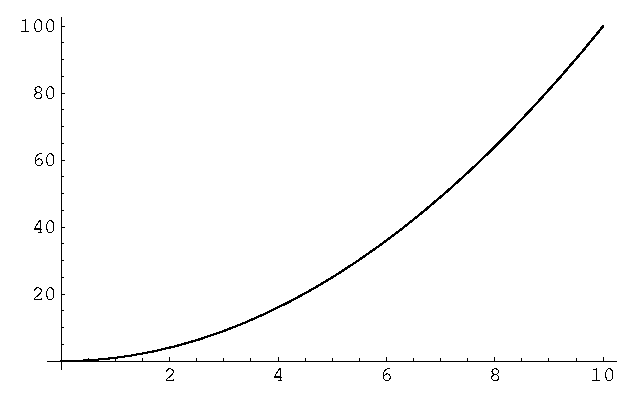
\includegraphics{plot.eps}
  \caption{%
    By default figures are not centered.
    This is a long caption to demonstrate that captions are single spaced.
  }
  \label{fi:not-centered}
\end{figure}

\Repeat{This is the second paragraph.}{10}

\begin{figure}[h]
  \centering
  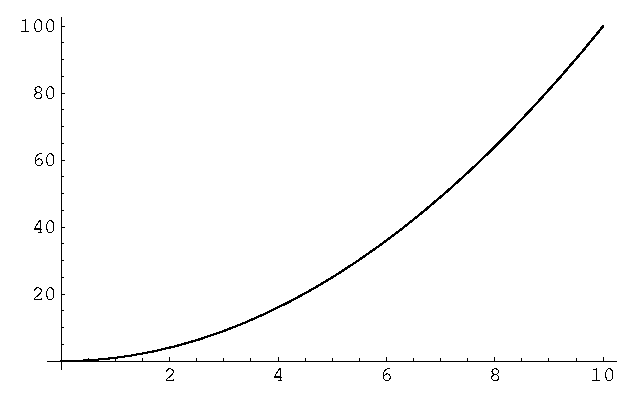
\includegraphics{plot.eps}
  \caption{Use {\tt \char'134centering\/} to center figures.}
  \label{fi:centered}
\end{figure}

\Repeat{This is the third paragraph.}{15}

\begin{figure}[h]
  \centering
  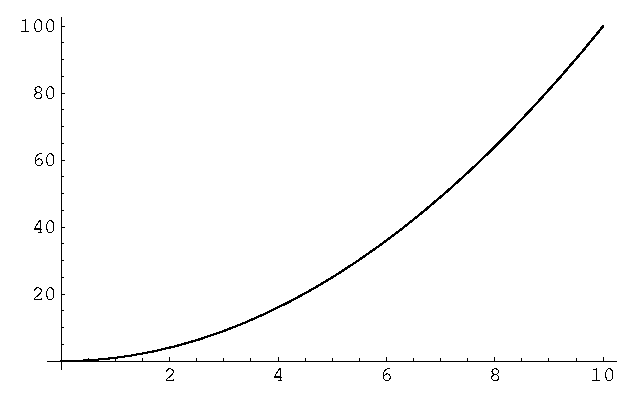
\includegraphics{plot.eps}
  \caption{This is another figuure.}
  \label{fi:another}
\end{figure}

\Repeat{This is the fourth paragraph.}{10}

\begin{figure}[h]
  \centering 
  \subfigure[First subcaption.]{\label{sf:two-parts-a}  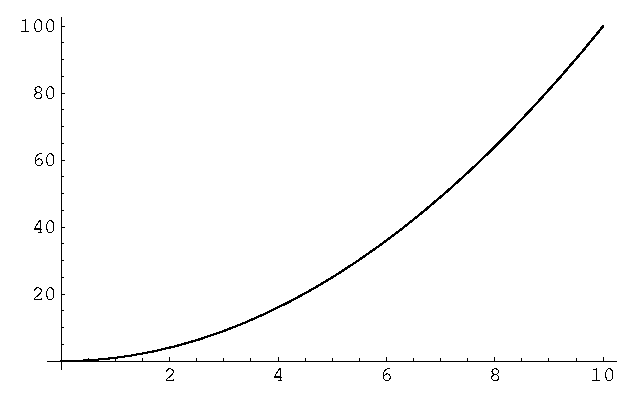
\includegraphics[width=0.3\textwidth]{plot.eps}}%
  \hskip 0.5truein
  \subfigure[Second subcaption.]{\label{sf:two-parts-b}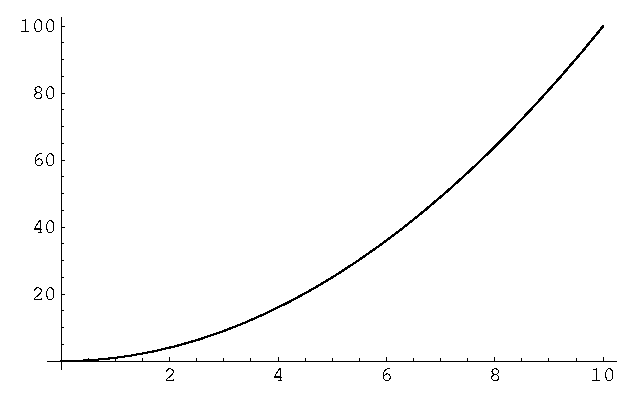
\includegraphics[width=0.3\textwidth]{plot.eps}}
  \caption{This figure has two parts.}
  \label{fi:two-parts}
\end{figure}

\Repeat{This is the fifth paragraph.}{10}

\begin{figure}[h]
  \centering
  \subfigure[First subcaption.]{\label{sf:four-parts-a}  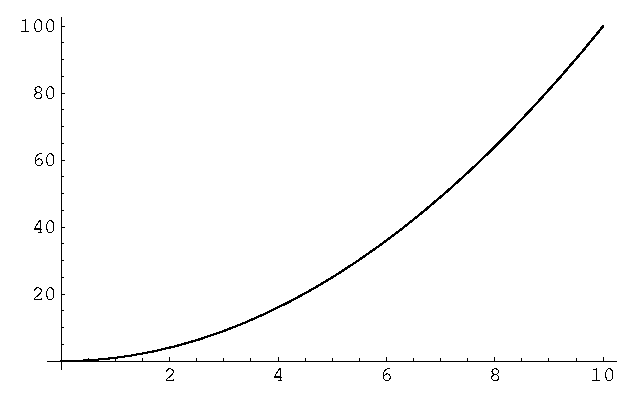
\includegraphics[width=0.3\textwidth]{plot.eps}}%
  \hskip 0.5truein
  \subfigure[Second subcaption.]{\label{sf:four-parts-b}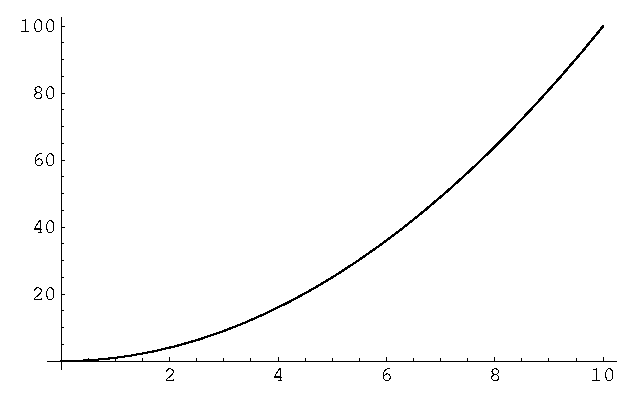
\includegraphics[width=0.3\textwidth]{plot.eps}}
  \subfigure[Third subcaption.]{\label{sf:four-parts-c}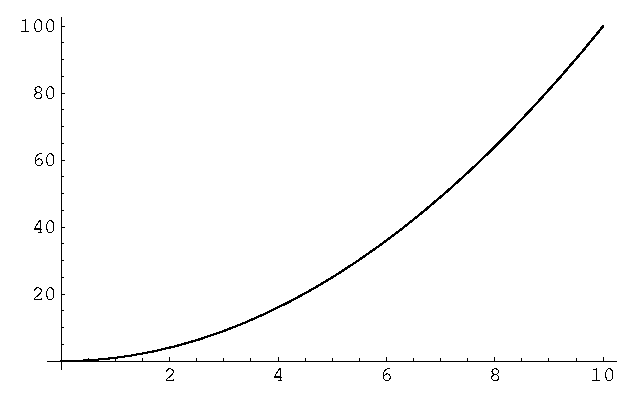
\includegraphics[width=0.3\textwidth]{plot.eps}}%
  \hskip 0.5truein
  \subfigure[Fourth subcaption.]{\label{sf:four-parts-d}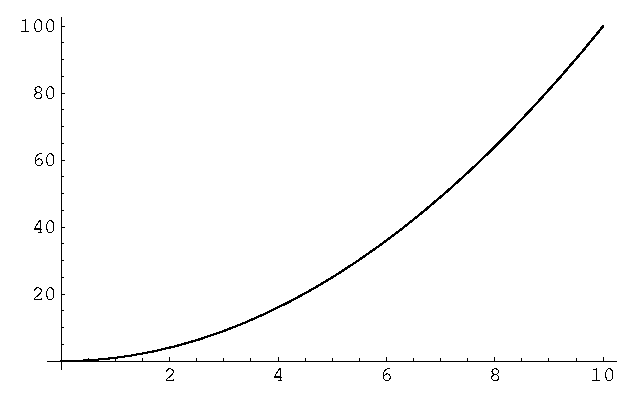
\includegraphics[width=0.3\textwidth]{plot.eps}}
  \caption{This figure has four parts.}
  \label{fi:four-parts}
\end{figure}

\Repeat{This is the sixth paragraph.}{10}

%
%  THIS FILE DOES SOME UNUSUAL THINGS TO MAKE
%  IT EASIER TO DO DEMONSTRATIONS.  IT SHOULD
%  NOT BE USED AS AN EXAMPLE OF HOW TO PREPARE
%  A FILE.  SEE THE OUTPUT OF THIS FOR LATEX
%  INPUT AND OUTPUT EXAMPLES.
%




%
%  demo-mathematics.tex  2008-12-09  Mark Senn  http://engineering.purdue.edu/~mark
%

\chapter{Demonstrate Mathematics}

    % Use single spacing.
    \Baselinestretch{1}

    % You don't normally need this.
    \mbox{}

    \begin{verbatim}
% From _More Math Into LaTeX_, 4th Edition, page 152:
%     TeX uses $$ to open and close a displayed math environment.
%     In LaTeX, this may occassionally cause problems.  Don't do it.
\[
    E = mc^2
\]
    \end{verbatim}
% From _More Math Into LaTeX_, 4th Edition, page 152:
%     TeX uses $$ to open and close a displayed math environment.
%     In LaTeX, this may occassionally cause problems.  Don't do it.
\[
    E = mc^2
\]
    \vskip\baselineskip
    \hrule
    \vskip0.5\baselineskip
    \filbreak

    \begin{verbatim}
\begin{equation}
    E = mc^2
\end{equation}
    \end{verbatim}
\begin{equation}
    E = mc^2
\end{equation}
    \vskip\baselineskip
    \hrule
    \vskip0.5\baselineskip
    \filbreak

    \begin{verbatim}
% Mydefs.tex defines \be to be \begin{equation} and
% \ee to be \end{equation}.
\be
    E = mc^2
\ee
    \end{verbatim}
% Mydefs.tex defines \be to be \begin{equation} and
% \ee to be \end{equation}.
\be
    E = mc^2
\ee
    \vskip\baselineskip
    \hrule
    \vskip0.5\baselineskip
    \filbreak

    \begin{verbatim}
\be
    x = -\frac{b}{2a} \pm \frac{\sqrt{b^2 - 4ac}}{2a}
\ee
    \end{verbatim}
\be
    x = -\frac{b}{2a} \pm \frac{\sqrt{b^2 - 4ac}}{2a}
\ee
    \vskip\baselineskip
    \hrule
    \vskip0.5\baselineskip
    \filbreak

    \begin{verbatim}
% requires \usepackage{amsmath}; use align* for no equation number
\begin{align}
    a = {}& b + c\\
    x = {}& y + z
\end{align}
    \end{verbatim}
% requires \usepackage{amsmath}; use align* for no equation number
\begin{align}
    a = {}& b + c\\
    x = {}& y + z
\end{align}
    \vskip\baselineskip
    \hrule
    \vskip0.5\baselineskip
    \filbreak

    \begin{verbatim}
\[
    Z = \left(
        \begin{array}{cc}
            a& b\\
            c& d
        \end{array}
    \right)
\]
    \end{verbatim}
\[
    Z = \left(
        \begin{array}{cc}
            a& b\\
            c& d
        \end{array}
    \right)
\]
    \vskip\baselineskip
    \hrule
    \vskip0.5\baselineskip
    \filbreak

    \begin{verbatim}
\begin{equation}
    \begin{split}
        a = {}& b + c\\
            {}& + d + e
    \end{split}      
\end{equation}
    \end{verbatim}
\begin{equation}
    \begin{split}
        a = {}& b + c\\
            {}& + d + e
    \end{split}      
\end{equation}
    \vskip\baselineskip
    \hrule
    \vskip0.5\baselineskip
    \filbreak

    \begin{verbatim}
\be
    (\cos x)^2 + (\sin x)^2 = 1
\ee
    \end{verbatim}
\be
    (\cos x)^2 + (\sin x)^2 = 1
\ee
    \vskip\baselineskip
    \hrule
    \vskip0.5\baselineskip
    \filbreak

    \begin{verbatim}
If $X = \cos x$ and $Y = \sin x$ then $X^2 + Y^2 = 1$.
    \end{verbatim}
If $X = \cos x$ and $Y = \sin x$ then $X^2 + Y^2 = 1$.
    \vskip\baselineskip
    \hrule
    \vskip0.5\baselineskip
    \filbreak

%
%  demo-multicols.tex  2007-03-19  Mark Senn  http://www.ecn.purdue.edu/~mark
%
%  Demonstrate multicols.
%
%  The multicols package must be loaded for this to work.
%  To load the multicols package put
%      \usepackage{multicols}
%  between the "\documentclass" and "\begin{document}" commands.
%

\chapter{Demonstrate Multicols}

% Put this amount of space between the columns.
\setlength{\columnsep}{0.5truein}

% Separate the columns with a vertical rule this wide.
\setlength{\columnseprule}{0.4pt}

\Repeat{This is one column.}{25}

\begin{multicols}{2}
\Repeat{This is two columns.}{25}
\end{multicols}

\begin{multicols}{3}
\Repeat{This is three columns.}{25}
\end{multicols}

\begin{multicols}{4}
\Repeat{This is four columns.}{25}
\end{multicols}

\begin{multicols}{5}
\Repeat{This is five columns.}{25}
\end{multicols}

%
%  demo-tables.tex  2014-08-08  Mark Senn
%
%  Demonstrate how to do tables.
%

\chapter{Demonstrate Tables}

% \newlength{\ta}
% \newlength{\tb}
% \newlength{\tc}
% 
% \settowidth{\ta}{\vbox{\hbox{Money}\hbox{Market}}}
% \settowidth{\tb}{\vbox{\hbox{Stocks}\hbox{and}\hbox{Bonds}}}
% \settowidth{\tc}{\vbox{\hbox{Money}\hbox{Market}\hbox{and}\hbox{Stocks}}}
% 
% {
%     \renewcommand{\baselinestretch}{1}
%     \begin{table}
%       \caption{%
%         \hfil Allocation of the IRA and Keogh Wealth\hfil\break
%         \mbox{}\hfil for Investors With or Without Brokerage Accounts\hfil
%       }
%       \label{tab:ira}
%       \begin{center}
%         \begin{tabular}%
%           {%
%             |%
%             c%
%             |%
%             >{\centering\hspace{0pt}}m{\the\ta}%  Money Market
%             |%
%             c%                                    Stocks 
%             |%
%             c%                                    Bonds
%             |%
%             c%                                    Diversified
%             |%
%             >{\centering\hspace{0pt}}m{\the\tb}%  Stocks and Bonds
%             |%
%             >{\centering\hspace{0pt}}m{\the\tc}%  Money Market and Stocks
%             |%
%             c%                                    Others
%             |%
%           }
%           \hline
%           IMP&
%             Money Market&
%             Stocks&
%             Bonds&
%             Diversified&
%             Stocks and Bonds&
%             Money Market and Stocks&
%             Others\tabularnewline
%           \hline
%           1& 14.19\%& 57.71\%& 12.21\%& 4.50\%& 7.36\%& 3.04\%& 0.99\%\tabularnewline \hline
%           2& 14.08\%& 58.18\%& 12.32\%& 4.44\%& 7.30\%& 2.80\%& 0.88\%\tabularnewline \hline
%           3 &14.26\%& 58.09\%& 12.27\%& 4.50\%& 7.19\%& 2.75\%& 0.94\%\tabularnewline \hline
%           4 &13.94\%& 58.11\%& 12.14\%& 4.78\%& 7.35\%& 2.68\%& 0.99\%\tabularnewline \hline
%           5 &13.92\%& 58.13\%& 11.93\%& 4.56\%& 7.60\%& 2.98\%& 0.88\%\tabularnewline \hline
%         \end{tabular}
%       \end{center}
%       This table presents the allocations of the wealth in the IRA
%       and Keogh accounts in various asset classes.
%       Results from each set of imputed data are presented here.
%       The first column lists the number of the imputations,
%       and rest of the columns lists various allocations.
%       Entrees under each asset class show the percentage of investors
%       who have most of their IRA
%       and Keogh wealth invested in that particular asset class.
%       The asset class Diversified
%       includes stocks,
%       bonds,
%       and money market investments.
%       The asset class Others
%       include investments in various life insurance products,
%       annuities,
%       real estate, etc.
%       \medskip
%     \footnotesize SOURCE: Survey of Consumer Finances,
%     2001,
%     Federal Reserve Board,
%     USA.\par
%   \end{table}
% }

Here is a really simple table.

% "h" means put table here---don't let it float to top or bottom of page
\begin{table}[h]
  \caption{American Presidents}
  \begin{center}
    \begin{tabular}{rl}
      \bf Number& \bf Name\\
      1& George Washington\\
      2& John Adams\\
      3& Thomas Jefferson\\
    \end{tabular}
  \end{center}
  \label{ta:American-Presidents}
\end{table}

There are 72.27 points per inch.
I like to put 2 points of vertical space between the heading
(Number Name)
and the first line
(1 George Washington)
of the table.

\begin{table}[h]
  \caption{American Presidents with 2pt vertical space after heading}
  \begin{center}
    \begin{tabular}{rl}
      \bf Number& \bf Name\\[2pt]  % put 2pt vertical space after this line
      1& George Washington\\
      2& John Adams\\
      3& Thomas Jefferson\\
    \end{tabular}
  \end{center}
  \label{ta:American-Presidents-with-2pt}
\end{table}

\LaTeX\ can print horizontal and vertical rules in tables.
I don't like the way this looks.

\begin{table}[h]
  \caption{American Presidents with horizontal and vertical lines}
  \begin{center}
    % "|" prints a vertical rule, "c" means center
    \begin{tabular}{|c|l|}
      % "\hline" prints a horizontal rule
      \hline
      \bf\#& \bf Name\\
      \hline
      1& George Washington\\
      \hline
      2& John Adams\\
      \hline
      3& Thomas Jefferson\\
      \hline
    \end{tabular}
  \end{center}
  \label{ta:American-Presidents-with-horizontal}
\end{table}

\newpage

Here is a more complicated table.

\begin{table}[h]
  \caption{C Bitwise Operators}
  \begin{center}
    % "|" prints a vertical rule, "c" means center
    \begin{tabular}{cccc}
      \bf A& \bf B& \bf A$|$B& \bf A\&B\\[2pt]
      0& 0& 0& 0\\
      0& 1& 1& 0\\
      1& 0& 1& 0\\
      1& 1& 1& 1\\
    \end{tabular}
  \end{center}
  \label{ta:C-Bitwise}
\end{table}

You can use Plain \TeX's \verb+\halign+ command to make tables also.
If you can't do a complicated table using \LaTeX\ commands
you may want to try using Plain \TeX\ commands.
\LaTeX's table making commands use Plain \TeX\ commands.

\begin{table}[h]
  \caption{American Presidents using {\tt\char'134 halign}}
  \hbox to \textwidth{\hss\vbox{\halign{%
    \strut #&      % 0. \strut
    \hfil#\qquad&  % 1. Number
    #\hfil\cr      % 2. Name
    %
    & \bf Number& \bf Name\cr
    \noalign{\vskip 2pt}
    & 1& George Washington\cr
    & 2& John Adams\cr
    & 3& Thomas Jefferson\cr
  }}\hss}
  \label{ta:American-Presidents-using}
\end{table}

The next page shows how to do a table that is too long to fit on one page.

\newpage

% This is loosely based on page 106 of _A Guide to LaTeX_, third edition,
% by Helmut Kopka and Patrick W. Daly.
\begin{longtable}{|l|l|}
    \caption{State Abbreviations}\\
    \hline
    State& Abbreviation\\
    \hline
  \endfirsthead
    \caption[]{\emph{continued}}\\
    \hline
    State& Abbreviation\\
    \hline
  \endhead
    \hline
    \multicolumn{2}{r}{\emph{continued on next page}}
  \endfoot
    \hline
  \endlastfoot
  Alabama& AL\\
  Alaska& AK\\
% American Samoa& AS\\
  Arizona& AZ\\
  Arkansas& AR\\
% Armed Forces Europe& AE\\
% Armed Forces Pacific& AP\\
% Armed Forces the Americas& AA\\
  California& CA\\
  Colorado& CO\\
  Connecticut& CT\\
  Delaware& DE\\
% District of Columbia& DC\\
% Federated States of Micronesia& FM\\
  Florida& FL\\
  Georgia& GA\\
% Guam& GU\\
  Hawaii& HI\\
  Idaho& ID\\
  Illinois& IL\\
  Indiana& IN\\
  Iowa& IA\\
  Kansas& KS\\
  Kentucky& KY\\
  Louisiana& LA\\
  Maine& ME\\
% Marshall Islands& MH\\
  Maryland& MD\\
  Massachusetts& MA\\
  Michigan& MI\\
  Minnesota& MN\\
  Mississippi& MS\\
  Missouri& MO\\
  Montana& MT\\
  Nebraska& NE\\
  Nevada& NV\\
  New Hampshire& NH\\
  New Jersey& NJ\\
  New Mexico& NM\\
  New York& NY\\
  North Carolina& NC\\
  North Dakota& ND\\
% Northern Mariana Islands& MP\\
  Ohio& OH\\
  Oklahoma& OK\\
  Oregon& OR\\
  Pennsylvania& PA\\
% Puerto Rico& PR\\
  Rhode Island& RI\\
  South Carolina& SC\\
  South Dakota& SD\\
  Tennessee& TN\\
  Texas& TX\\
  Utah& UT\\
  Vermont& VT\\
% Virgin Islands& VI\\
  Virginia& VA\\
  Washington& WA\\
  West Virginia& WV\\
  Wisconsin& WI\\
  Wyoming& WY\\
\end{longtable}

\newcommand{\cbackslash}{\char'134}
\newcommand{\copencurly}{\char'173}
\newcommand{\cclosecurly}{\char'175}

\newlength{\twidth}
\newlength{\theight}

\setlength{\twidth}{\textwidth}
\setlength{\theight}{\textheight}

\begin{sidewaystable}
  % The following two lines compensate for what I think is a bug.
  \setlength{\textwidth}{\theight}
  \setlength{\textheight}{\twidth}
  \caption{%
    sidewaystable
    {\tt\cbackslash begin\copencurly tabular\cclosecurly\/}%
    \ldots
    {\tt\cbackslash end\copencurly tabular\cclosecurly\/}%
  }
  \begin{center}
    \begin{tabular}{rl}
      \bf Number& \bf Name\\[2pt]  % put 2pt vertical space after this line
      1& George Washington\\
      2& John Adams\\
      3& Thomas Jefferson\\
    \end{tabular}
  \end{center}
\end{sidewaystable}

\begin{sidewaystable}
  % The following two lines compensate for what I think is a bug.
  \setlength{\textwidth}{\theight}
  \setlength{\textheight}{\twidth}
  \caption{%
    sidewaystable
    {\tt\cbackslash halign\copencurly}\ldots{\tt\cclosecurly\/} table%
  }
  \hbox to \textwidth{\hss\vbox{\halign{%
    \strut #&      % 0. \strut
    \hfil#\qquad&  % 1. Number
    #\hfil\cr      % 2. Name
    %
    & \bf Number& \bf Name\cr
    \noalign{\vskip 2pt}
    & 1& George Washington\cr
    & 2& John Adams\cr
    & 3& Thomas Jefferson\cr
  }}\hss}
\end{sidewaystable}

%\newlength{\ta}
%\settowidth{\ta}{\vbox{\hbox{Money}\hbox{Market}}}
%\newlength{\tb}
%\settowidth{\tb}{\vbox{\hbox{Stocks}\hbox{and}\hbox{Bonds}}}
%\newlength{\tc}
%\settowidth{\tc}{\vbox{\hbox{Money}\hbox{Market}\hbox{and}\hbox{Stocks}}}
%
%  {\renewcommand{\baselinestretch}{1}
%\begin{table}
%  \caption{\hfil Allocation of the IRA and Keogh Wealth\hfil\break\mbox{}\hfil for Investors With or Without Brokerage Accounts\hfil}
%  \label{tab:ira}
%  \begin{center}
%    \begin{tabular}%
%      {%
%        |%
%        c%
%        |%
%        >{\centering\hspace{0pt}}m{\the\ta}%  Money Market
%        |%
%        c%                                    Stocks 
%        |%
%        c%                                    Bonds
%        |%
%        c%                                    Diversified
%        |%
%        >{\centering\hspace{0pt}}m{\the\tb}%  Stocks and Bonds
%        |%
%        >{\centering\hspace{0pt}}m{\the\tc}%  Money Market and Stocks
%        |%
%        c%                                    Others
%        |%
%      }
%      \hline
%      IMP&
%        Money Market&
%        Stocks&
%        Bonds&
%        Diversified&
%        Stocks and Bonds&
%        Money Market and Stocks&
%        Others\tabularnewline
%      \hline
%      1& 14.19\%& 57.71\%& 12.21\%& 4.50\%& 7.36\%& 3.04\%& 0.99\%\tabularnewline \hline
%      2& 14.08\%& 58.18\%& 12.32\%& 4.44\%& 7.30\%& 2.80\%& 0.88\%\tabularnewline \hline
%      3 &14.26\%& 58.09\%& 12.27\%& 4.50\%& 7.19\%& 2.75\%& 0.94\%\tabularnewline \hline
%      4 &13.94\%& 58.11\%& 12.14\%& 4.78\%& 7.35\%& 2.68\%& 0.99\%\tabularnewline \hline
%      5 &13.92\%& 58.13\%& 11.93\%& 4.56\%& 7.60\%& 2.98\%& 0.88\%\tabularnewline \hline
%    \end{tabular}
%  \end{center}
%  This table presents the allocations of the wealth in the IRA
%  and Keogh accounts in various asset classes.
%  Results from each set of imputed data are presented here.
%  The first column lists the number of the imputations,
%  and rest of the columns lists various allocations.
%  Entrees under each asset class show the percentage of investors
%  who have most of their IRA
%  and Keogh wealth invested in that particular asset class.
%  The asset class Diversified
%  includes stocks,
%  bonds,
%  and money market investments.
%  The asset class Others
%  include investments in various life insurance products,
%  annuities,
%  real estate, etc.
%  \medskip
%  \footnotesize SOURCE: Survey of Consumer Finances,
%  2001,
%  Federal Reserve Board,
%  USA.\par
%\end{table}
%  }


%
%  demo-text.tex  2007-07-17  Mark Senn  http://engineering.purdue.edu/~mark
%

\chapter{Demonstrate Text}

% Use single spacing.
\Baselinestretch{1}

% You don't normally need this.
\mbox{}


%\vbox{
\begin{verbatim}
This is a sentence.
This is a sentence.
This is a sentence.
This is a sentence.
This is a sentence.

This is a sentence.
This is a sentence.
This is a sentence.
This is a sentence.
This is a sentence.
\end{verbatim}
This is a sentence.
This is a sentence.
This is a sentence.
This is a sentence.
This is a sentence.

This is a sentence.
This is a sentence.
This is a sentence.
This is a sentence.
This is a sentence.
\vskip\baselineskip
\hrule
%}
\vskip0.5\baselineskip
\filbreak

%\vbox{
\begin{verbatim}
From \verb+http://www.biblegateway.com/passage/?book_id=1&chapter=1&version=50+:

\begin{quote}
    1 In the beginning God created the heavens and the earth.
    2 The earth was without form,
    and void;
    and darkness was on the face of the deep.
    And the Spirit of God was hovering over the face of the waters.

    3 Then God said,``Let there be light'';
    and there was light.
    4 And God saw the light,
    that it was good;
    and God divided the light from the darkness.
    5 God called the light Day,
    and the darkness He called Night.
    So the evening and the morning were the first day. 
\end{quote}
\end{verbatim}
From \verb+http://www.biblegateway.com/passage/?book_id=1&chapter=1&version=50+:

\begin{quote}
    1 In the beginning God created the heavens and the earth.
    2 The earth was without form,
    and void;
    and darkness was on the face of the deep.
    And the Spirit of God was hovering over the face of the waters.

    3 Then God said,``Let there be light'';
    and there was light.
    4 And God saw the light,
    that it was good;
    and God divided the light from the darkness.
    5 God called the light Day,
    and the darkness He called Night.
    So the evening and the morning were the first day. 
\end{quote}
\vskip\baselineskip
\hrule
%}
\vskip0.5\baselineskip
\filbreak

%\vbox{
\begin{verbatim}
\begin{description}
    \item[apple]
        A red fruit.
    \item[banana]
        A yellow fruit.
        This sentence is to make the entry longer so you can see what happens.
        This sentence is to make the entry longer so you can see what happens.
    \item[cherry]
        A red friut.
\end{description}
\end{verbatim}
\begin{description}
    \item[apple]
        A red fruit.
    \item[banana]
        A yellow fruit.
        This sentence is to make the entry longer so you can see what happens.
        This sentence is to make the entry longer so you can see what happens.
    \item[cherry]
        A red friut.
\end{description}
\vskip\baselineskip
\hrule
%}
\vskip0.5\baselineskip
\filbreak

%\vbox{
\begin{verbatim}
\begin{enumerate}
    \item apple
    \item banana
        This sentence is to make the entry longer so you can see what happens.
        This sentence is to make the entry longer so you can see what happens.
    \item cherry
\end{enumerate}
\end{verbatim}
\begin{enumerate}
    \item apple
    \item banana
        This sentence is to make the entry longer so you can see what happens.
        This sentence is to make the entry longer so you can see what happens.
    \item cherry
\end{enumerate}
\vskip\baselineskip
\hrule
%}
\vskip0.5\baselineskip
\filbreak


%\vbox{
\begin{verbatim}
\begin{itemize}
    \item apple
    \item banana
        This sentence is to make the entry longer so you can see what happens.
        This sentence is to make the entry longer so you can see what happens.
    \item cherry
\end{itemize}
\end{verbatim}
\begin{itemize}
    \item apple
    \item banana
        This sentence is to make the entry longer so you can see what happens.
        This sentence is to make the entry longer so you can see what happens.
    \item cherry
\end{itemize}
\vskip\baselineskip
\hrule
%}
\vskip0.5\baselineskip
\filbreak



% Notes and footnotes are optional.
% Reference: TM2006 page 34.
% I have not implemented this yet.  Mark Senn 2002-06-03
%%\include{notes}

% A vita is optional for masters theses
% and required for doctoral dissertations.
% Reference: TM2006 page 13.
% CHANGE NEXT LINE?
%
%  vita.tex   2003.07.23  14:59:33   Mark Senn <mds@purdue.edu>
%
%  This is the vita for a simple, example thesis.
%
%  A vita is required only in a doctoral dissertation.
%

\begin{vita}
    [Put a brief autobiographical sketch here.]
\end{vita}


\end{document}

% LaTeX won't read after the \end{document} command.
% You can put notes to yourself or LaTeX input not
% ready for use here if you'd like.
